%!TEX TS-program = pdflatex
\documentclass[a4paper,12pt,twoside]{article}

\usepackage{mathptmx}
\usepackage{parskip}
\usepackage[top=1.5in,left=1in,right=1in,bottom=1in]{geometry}
%\setlength{\parindent}{0pt}
%\setlength{\parskip}{\the\baselineskip}

\usepackage{subcaption}
\usepackage{booktabs}

% JT: I've commented this out so that we can see page numbers while writin
%\pagestyle{empty} 

\newcommand{\mcdm}[1]{\textbf{\color{blue}[mcdm: #1]}}

\makeatletter
\renewcommand\@makefntext[1]{%
  \parindent 1em\noindent
  \hbox{\@makefnmark}#1}
\renewcommand\large{\@setfontsize\large{14pt}{18}} % For standardizing with the Word template: normally \large is 14.4pt
\makeatother
\usepackage{titlesec}
\titleformat{\subsection}{\normalfont\normalsize}{\thesubsection.}{1ex}{}
\titleformat{\subsubsection}{\normalfont\normalsize}{\thesubsubsection.}{1ex}{}
\titleformat{\section}{\normalfont\normalsize\bfseries}{\thesection.}{1ex}{}
% \titlespacing*{\section}{0pt}{*0}{0pt}
% \titlespacing*{\subsection}{0pt}{\the\baselineskip}{0pt}

\usepackage[longnamesfirst]{natbib} 
%\bibpunct{(}{)}{;}{a}{,}{,}
\bibpunct{(}{)}{,}{a}{,}{,}

\setlength{\bibsep}{0pt} \relax
\setcitestyle{notesep={: },yysep={, }} \relax

\usepackage{linguex,url}
\def\refdash{} % To suppress the dash in (2-a) etc. Defining both as different versions of linguex had different names for this command.
\def\firstrefdash{}


\usepackage{titleps}
\usepackage{lipsum}
\newpagestyle{mystyle}{
\sethead[\thepage][\Author][]{}{\Title}{\thepage}
}
\pagestyle{mystyle}
\author{Hofmann \and de Marneffe  \and Tonhauser}
%\title{Projection variation of clausal complements across different operators}
\title{Projection variation: Is the family of sentences really a family?}
\makeatletter
\newcommand\Author{Hofmann, de Marneffe, and Tonhauser}
\let\Title\@title
\makeatother
%header with author and title

% JT commented out whle editing
%\pagenumbering{gobble} 
%suppresses page numbering in header


%% other packages I added (LH)
% misc formatting
	\usepackage{booktabs}
    \usepackage[export]{adjustbox}
    \usepackage{rotating}
    \usepackage{longtable}

%% bibliography
	\newcommand{\posscite}[1]{\citeauthor{#1}'s (\citeyear{#1})}

 \newcommand{\poscite}[1]{\citeauthor{#1}'s \citeyear{#1}}

% drawing
	\usepackage{graphicx}
	\usepackage{xcolor}
    \definecolor{op-n-color}{HTML}{009E73}
    \definecolor{op-m-color}{HTML}{0072B2}
    \definecolor{op-c-color}{HTML}{404040}
    \definecolor{op-q-color}{HTML}{E69F00}
    \definecolor{pred-fcv-color}{HTML}{CC79A7}


\begin{document}
%%\maketitle
\setlength{\Extopsep}{0pt}
\thispagestyle{empty}

{\large \textbf{Projection variation: Is the family of sentences really a family?}}\footnote{We thank Taylor Mahler for assistance in collecting the data presented here as well as valuable comments. We gratefully acknowledge the National Science Foundation grant BCS \#1452674 (to Marie-Catherine de Marneffe, Craige Roberts, and Judith Tonhauser), which provided financial support for this project.}\\
Lisa HOFMANN --- \textit{University of Stuttgart}\\
Marie-Catherine DE MARNEFFE --- \textit{UCLouvain}\\
Judith TONHAUSER --- \textit{University of Stuttgart}\\

\textbf{Abstract.}
    Under the `family of sentences' diagnostic for projection, the projection of content is investigated by embedding the expression that contributes the content in the scope of negation, polar questions, epistemic possibility modals, and conditional antecedents. This paper reports on the results of a set of experiments designed to investigate whether there is variation in the projection of content from under these four types of entailment-canceling operators. The contents investigated are the contents of the complements of 20 English clause-embedding predicates. The results of the experiments suggest (i) that the by-operator variation is small when aggregating over the 20 contents, but (ii) that the effect of operator differs between the clause-embedding predicates. The results of these experiments also extend a result of \citealt{degen_are_2022}, that projection ratings in polar questions do not categorically distinguish factive from non-factive predicates, to cases with negation, the epistemic possibility modal \textit{perhaps}, and conditional antecedents. The observed by-predicate and by-operator variation is not captured by existing theoretical accounts of projection (e.g., \citealt{heim_projection_1983,van_der_sandt_presupposition_1992,abrusan_predicting_2011,schlenker_triggering_2021}). Our results suggest that an empirically adequate projection analysis must consider interactions between predicates and operators. 

\textbf{Keywords:} Projection variation, entailment-canceling operators, (non)factive predicates. 

\section{Introduction} \label{sec:intro}
    The `family of sentences' diagnostic is the standard way of diagnosing whether a content is projective (e.g., \citealt{chierchia_meaning_1990}). For instance, in \ref{ex:simple}, the content of the clausal complement of \emph{discover} (that Julian dances salsa) is diagnosed as projective content, if it is typically implied not just by an utterance of \ref{ex:simple}, but also by utterances of the variants in \ref{ex:family}, where \ref{ex:simple} is embedded under an entailment-canceling operator, such as negation \ref{ex:neg}, a polar question \ref{ex:q}, an epistemic possibility modal \ref{ex:mod}, or in a conditional antecedent \ref{ex:cond}.

    \ex.\label{ex:simple} Cole discovered that Julian dances salsa.

	\ex. \label{ex:family}
		\a. \label{ex:neg}
			{\bf Negation:} \hfill
			Cole didn't discover that Julian dances salsa.
		\b. \label{ex:q}
			{\bf Polar Question:} \hfill
			Did Cole discover that Julian dances salsa?
		\c. \label{ex:mod}
			{\bf Modal:} \hfill
			Perhaps Cole discovered that Julian dances salsa.
		\d. \label{ex:cond}
			{\bf Conditional:} \hfill
			If Cole discovered that Julian dances salsa, Logan will be joyful.
		\z.
	\z.

    Some research, however, suggests that entailment-canceling operators may affect projection differentially. For instance, \citet{karttunen_observations_1971} proposed distinguishing English factive predicates (e.g., \textit{regret}) from semi-factives (e.g., \textit{discover}). Based on \Next, he argued that the content of the complement (CC) of true factives consistently projects across the operators in \Last, but that of semi-factives does not always project from under polar questions, modals, or conditionals.%

    \ex. \citealt{karttunen_observations_1971}: (22, 24--26)
        \a. John didn't \{regret/discover\} that he had not told the truth.
        \b. Did you \{regret/discover\} that you had not told the truth?
        \b. If I \{regret/discover\} later that I have not told the truth, I will confess it to everyone.
        \b. It is possible that I \{regret/discover\} later that I have not told the truth.
        \z.
    \z.

    There have been two experimental investigations of by-operator projection variation. First, \citet{smith_relationship_2014} investigated projection from under negation and conditional antecedents for various types of English projective contents. They found that the expressive content of epithets (e.g., \textit{idiot}) and the CC of \textit{know} was more projective under negation than conditionals. In contrast, the content of appositive relative clauses and the preparatory content of \textit{win} showed the opposite pattern, and the existential presupposition of clefts showed no difference.
    
    Second, \citet{sieker_projective_2022}  compared the projection of the CCs of German factives (\textit{wissen} `know', \textit{bereuen} `regret', \textit{ent\-hüllen} `reveal') and semi-factives (\textit{bemerken} `notice', \textit{entdecken} `discover', \textit{herausfinden} `find out') from under the four operators in \ref{ex:family}. Their results suggest that the CCs project more from under negation than from under the other three operators. Contrary to what \citet{karttunen_observations_1971} suggested, a comparison of the factive and semi-factive predicates did not reveal that the CCs of factive predicates project more from under polar questions, modals, or antecedents of conditionals than the CCs of semi-factive predicates.\footnote{The factive/semi-factive distinction is also called into question by naturally occurring examples where the CCs of factive predicates do not project from under the four operators (see \citealt{beaver_have_2010,de_marneffe_did_2012,de_marneffe_commitmentbank_2019}). For experimental research on the distinction, see \citealt{djarv_cognitive_2018}.
    }

    This paper reports on the results of a set of experiments that were designed to compare projection from under the four entailment-canceling operators in \ref{ex:family} in English. Our experiments extend the empirical scope of prior research on by-operator projection variation by investigating projection for a larger set of contents, namely the contents of the complements of the 20 English clause-embedding predicates in \ref{ex:predicates}, from \citet{degen_are_2022}.
    
    \ex. \label{ex:predicates}
    		\a. (Semi-)factive predicates: {\em be annoyed, know, reveal, discover, see}
      \b. Non-factive predicates: {\em acknowledge, admit, announce, confess, confirm, establish, hear, inform, prove, be right, demonstrate, pretend, say, suggest, think}
    
    The five predicates in \Last[a] have been characterized as factive or semi-factive. Our set of predicates also includes the 15 non-factives in \Last[b]. Including non-factive predicates in investigations of projection is motivated by the empirical investigations in \citealt{de_marneffe_commitmentbank_2019} and \citealt{degen_are_2022}, which suggest that the CCs of non-factives may also project and that projection ratings do not categorically distinguish factive and non-factive predicates.
  
    The results of our investigation suggest that the projection of the CCs of these 20 predicates is affected differently by the four entailment-canceling operators in \ref{ex:family},  but not in a way that is consistent with \poscite{karttunen_observations_1971} factive/semi-factive distinction. The results also replicate a result of \citealt{degen_are_2022}, namely that projection from under polar questions does not categorically distinguish factive and non-factive predicates. Finally, the results of our experiment extend this result of \citealt{degen_are_2022} to projection from under the other three entailment-canceling operators, thereby solidifying their claim that ``research on projective content has a much broader empirical scope than previously assumed'' (p.585), as this scope includes the CCs of both factive and non-factive predicates.


\section{Experiments}\label{s2}
	To assess the effect of entailment-canceling operator and clause-embedding predicate on projection, we collected projection judgments for the CCs of the 20 clause-embedding predicates in four sets of experiments.
    %
    The predicates were embedded under negation in Exps.~1, under polar questions in Exps.~2, under the epistemic possibility modal {\em perhaps} in Exps.~3, and in conditional antecedents in Exps.~4. Each set of experiments contained three experiments that differed in the at-issueness measure that was used in a separate block. In this paper, we limit our attention to the projection ratings collected in these twelve experiments.\footnote{\label{footnote-supplement}The experiments, data and analysis scripts, as well as the supplements referred to in this paper can be found in the following GitHub repository: \url{https://github.com/judith-tonhauser/CommitmentBankPlus}.}

	In all twelve experiments, projection was measured with the `certain that' diagnostic, which has been used to measure projection with both polar interrogative and declarative sentences (see, e.g., \citealt{tonhauser_prosodic_2016,djarv_prosodic_2017,stevens_rational_2017,tonhauser_how_2018,mahler_does_2019,mahler_social_2020,de_marneffe_commitmentbank_2019,sieker_projective_2022}).\footnote{For other diagnostics of projection see, e.g.\ \citealt{smith_projection_2011,xue_correlation_2011}, and \citealt{tonhauser_toward_2013}, and discussion in \citealt{tonhauser_how_2018}.}
    Under this diagnostic, participants are presented with utterances like those in \Next, and asked to rate whether the (named) speaker is certain of the CC. 

	\ex. \label{ex:certain-that}
		\a. Christopher: ``Cole didn't discover that Julian dances salsa.''
		\b. Christopher: ``Did Cole discover that Julian dances salsa?''
		\c. Christopher: ``Perhaps Cole discovered that Julian dances salsa.''
		\d. Christopher: ``If Cole discovered that Julian dances salsa, Logan will be joyful.''
		\z.
		Projection question: Is Christopher certain that Julian dances salsa?
	\z.

    We assume, following \citealt{tonhauser_how_2018} and \citealt{degen_are_2022}, that judgments of speaker certainty about the embedded content reflect speaker commitment to that content, that is, projection. If a participant interprets utterances like \Last[a--d] in a way that the speaker (here, Christopher) is certain of the CC, the CC is assumed to project. If a participant does not take the speaker to be certain of the CC, the CC is taken to not project.

    \paragraph{Participants.}
	    We recruited 250-300 participants for each of the 12 experiments. Participants for one experiment were recruited on Amazon's Mechanical Turk platform. These participants were required to have U.S.\ IP addresses and at least 99\% of previously approved HITs. Participants for the remaining experiments were recruited on Prolific. These participants were required to reside in the US, to be born in the US, to have English as their first language, and to have an approval rating of at least 99\%. See Supplement D (in the repository linked to in footnote \ref{footnote-supplement}) for further information about the participants. 
			

            \begin{figure}[h!]
				\centering
                    %\fbox{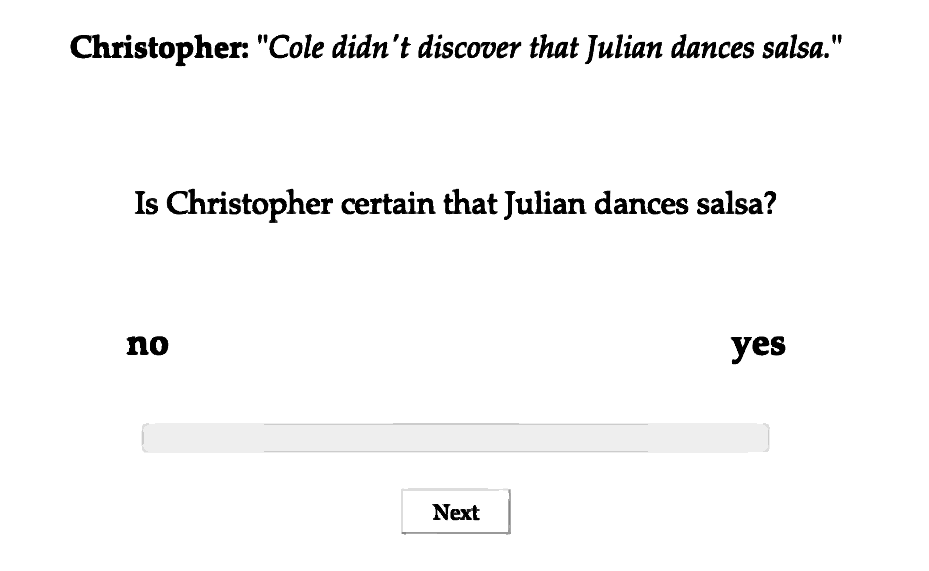
\includegraphics[scale=0.5]{task-1n-proj.eps}}
				\fbox{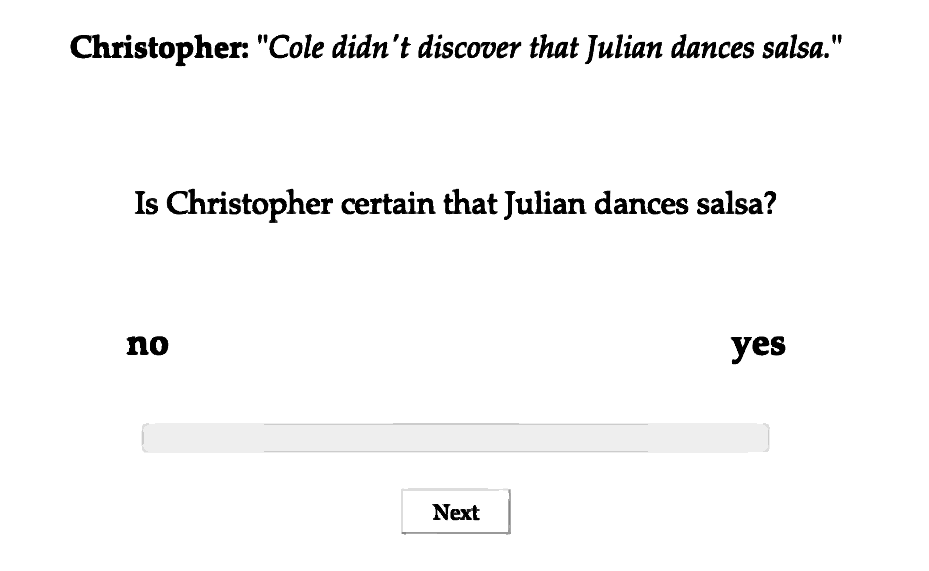
\includegraphics[width = .6\linewidth]{task-1n-proj.eps}}
				\caption{A sample trial from Exps.~1 (negation). In the other experiments, participants were presented with utterances with a different entailment-canceling operator.}
				\label{fig:trial}
			\end{figure}
   
		% \subsubsection{Materials}
        \paragraph{Materials.}
            The target sentences consisted of the 400 combinations of the 20 clause-em\-bed\-ding predicates in \ref{ex:predicates} with 20 embedded clauses (provided in Supplement A). As mentioned above, the predicates were embedded under negation in Exps.~1, under polar questions in Exps.~2, under the epistemic possibility modal \emph{perhaps} in Exps.~3, and in conditional antecedents in Exps.~4, for a total of 400 target stimuli in each of the four sets of experiments. To assess whether participants were attending to the task, each experiment included six control stimuli. For details on the six control stimuli, see Supplement C.

            Each participant saw a random set of 26 stimuli: Each set contained one target stimulus for each of the 20 clause-embedding predicates (each with a unique complement clause) and the same six control stimuli.\footnote{Each participant saw their set of 26 stimuli twice, once in the projection block and once in the at-issueness block. Block order was randomized. As mentioned above, we focus here on the projection ratings.} Trial order was randomized.
		
        %\subsubsection{Procedure}
        \paragraph{Procedure.}
            Participants were asked to imagine that they are at a party and that, when walking into the kitchen, they overhear somebody say something to somebody else.
            %
            On each trial, they read an utterance and gave a response to the `certain that' question on a slider marked `no' (coded as 0) at one end and `yes' (coded as 1) at the other. A sample trial %from Exps.~1
            is shown in Figure~\ref{fig:trial}.            
            Following \citealt{tonhauser_how_2018}, higher ratings of speaker certainty could reflect one of two things. First, higher certainty ratings could reflect greater speaker commitment towards the CC, and therefore greater projection. This assumes that speaker commitment is interpreted in a gradient way. Second, higher certainty ratings could reflect a higher probability that an interpreter takes the speaker to be committed to the CC.  On this interpretation, speaker commitment may be a binary, categorical property and projection variation is a result of uncertainty about speaker commitment. In this paper, we remain agnostic about the underlying interpretation of projectivity as a gradient property (for discussion, see  \citealt{grove_factivity_2023}).
            
            After completing the experiment, participants filled out a short optional demographic survey. To encourage truthful responses, participants were told that they would be paid no matter what answers they gave in the survey.

        %\subsubsection{Data exclusion}
        \noindent\textbf{Data exclusion.} Data were excluded based on self-declared non-native speaker status and other criteria given in Supplement D. The data from 2,682 participants entered into the analysis.
            % Data were excluded based on self-declared non-native speaker status and other criteria given in the Supplements \ref{app:d-participants}. The data from 2,682 participants entered into the analysis.

\section{Results and discussion}

        We first address by-operator variation (Section \ref{s:by-op}) and then the question of whether there is by-predicate variation in the observed by-operator variation (Section \ref{s:by-pred}). Finally, in Section \ref{s:factivity}, we relate our results to those of \citealt{degen_are_2022}, that projection from under polar questions does not categorically distinguish factive and non-factive predicates.
		
	\subsection{By-operator variation}\label{s:by-op}

        Figure~\ref{fig:op-ratings} shows the mean certainty ratings by entailment-canceling operator, aggregating over the clause-embedding predicates. As shown, there is projection variation by operator: The CCs of the clause-embedding predicates were relatively more projective when embedded in the antecedent of a conditional than in a polar interrogative, where they were relatively more projective than when they were embedded under negation or the epistemic modal {\em perhaps}.
        
            \begin{figure}[ht]
				\centering
				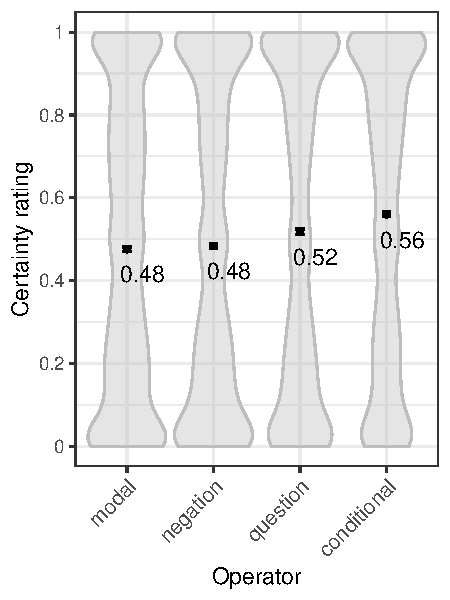
\includegraphics[scale = .7]{certainty-operator.pdf}
				\caption{Mean certainty ratings by operator. Error bars indicate $95\%$ bootstrapped confidence intervals. Violin plots indicate the kernel probability density of participants' individual ratings.
                }
				\label{fig:op-ratings}
			\end{figure}

        These observations are supported by a post-hoc pairwise comparison of the estimated means for each entailment-canceling operator using the \texttt{emmeans} package (\citealt{emmeans}) in R (\citealt{r}). The input to the pairwise comparison was a Bayesian mixed-effects beta regression model that was fit using the \texttt{brms} package (\citealt{buerkner2017}) with weakly informative priors. The model predicted certainty ratings\footnote{To model the certainty ratings using a beta regression, the ratings were first transformed from the interval [0,1] to the interval (0,1) using the method proposed in \citealt{smithson_better_2006}.} from a fixed effect of entailment-canceling operator (with treatment coding and `modal' as the reference level) and included a random by-predicate intercept.\footnote{See Supplement E for details on the model.} The output of the pairwise comparison were 95\% highest density intervals (HDIs) of estimated marginal mean differences between each of the operators. We assume that two operators differ in certainty ratings if the HDI of their pairwise comparison does not include 0. 

        Table~\ref{t:pairwise} provides the output of the pairwise comparison on a logit scale.
        As shown, the analysis suggests differences between each pair of operators. That is, certainty ratings are higher for CCs embedded in conditional antecedents than those embedded under polar questions, certainty ratings for CCs embedded under polar questions are higher than those for CCs embedded under negation, and finally certainty ratings for CCs embedded under negation are higher than those for CCs embedded under the epistemic modal \emph{perhaps}.

        \begin{table}[!h]
        \centering
        \begin{tabular}{lrrr}
        \toprule
         contrast & estimate & lower 95\% CrI & upper 95\% CrI \\\midrule
         conditional - negation & 0.21 & 0.18 & 0.24 \\ 
          conditional - question & 0.13 & 0.10 & 0.16 \\ 
          modal - conditional & -0.26 & -0.29 & -0.23 \\ 
          modal - negation & -0.05 & -0.08 & -0.02 \\ 
          modal - question & -0.14 & -0.17 & -0.11 \\ 
          negation - question & -0.09 & -0.12 & -0.06 \\ \bottomrule
        \end{tabular}
        \caption{Output of the pairwise comparison of entailment-canceling operators. The `contrast' column identifies entailment-canceling operators pairs, `estimate' the estimated marginal mean difference, and `lower/upper 95\% CrI' provide the lower/upper bounds of the HDIs.}\label{t:pairwise}
        \end{table}
        
        These results suggest that certainty ratings for the CCs of the English clause-embedding predicates we investigated vary by entailment-canceling operator. In contrast to \citealt{sieker_projective_2022} for German, the results of our experiments do not suggest that projection is strongest from under negation. Recall, however, that they only investigated projection of the CCs of (semi-) factive predicates. Since there is by-predicate variation in the effect of entailment-canceling operator on projection (as we show in the next section), this difference between the results of their experiment and ours might be due to the types of predicates investigated. Finally, the differences in mean certainty ratings between the four entailment-canceling operators are very small. This suggests that, when abstracting away from individual predicates and contents, projection from under the four entailment-canceling operators is very similar. In other words, when abstracting away from individual  contents, the family of sentences really are a family.
 
	\subsection{By-predicate variation in the effect of entailment-canceling operator}\label{s:by-pred}

        Figure~\ref{fig:op-pred-analysis} shows mean certainty ratings by entailment-canceling operator for the 20 predicates, with predicates ordered by their overall mean certainty rating. As shown, there is by-operator projection variation for each predicate. Further, the effect of operator differs between predicates. For instance, the five (semi-)factive predicates exhibit four different patterns.
        %
        First, the CC of \emph{be annoyed} projects
        most from under questions, less from under negation, followed by conditionals, and least from under the modal \emph{perhaps} (\textcolor{op-q-color}{Q} $>$ \textcolor{op-n-color}{N} $>$ \textcolor{op-c-color}{C} $>$ \textcolor{op-m-color}{M}).
        % more from under negation and questions than conditionals and the modal {\em perhaps};
        Second, the CC of \emph{know} projects most from under questions, less from conditionals and negation, and least from under {\em perhaps} (\textcolor{op-q-color}{Q} $> \{$\textcolor{op-n-color}{N}$,$ \textcolor{op-c-color}{C}$\} >$ \textcolor{op-m-color}{M}).
        %
        The CCs of \emph{discover} and \emph{see} exhibit a third pattern: They project most from under questions and conditionals, less from under negation, and least from under \emph{perhaps} ($\{$\textcolor{op-q-color}{Q}$,$ \textcolor{op-c-color}{C}$\}>$ \textcolor{op-n-color}{N} $>$ \textcolor{op-m-color}{M}).
        %
        Finally, the CC of \emph{reveal} projects most from conditionals, less from questions, and least from under negation and \emph{perhaps} (\textcolor{op-c-color}{C} $>$ \textcolor{op-q-color}{Q}  $> \{$\textcolor{op-m-color}{M}$, $\textcolor{op-n-color}{N}$\}$).
        %
        Thus, the CCs of none of our (semi-)factive predicts project uniformly from under all four entailment-canceling operators (contrary to what \citealt{karttunen_observations_1971} suggested for factive predicates) and the purported semi-factive predicates  \emph{discover} and \emph{reveal} do not project more from under negation than the other three entailment-canceling operators. 
        
         \begin{figure}[ht!]
            \centering
    		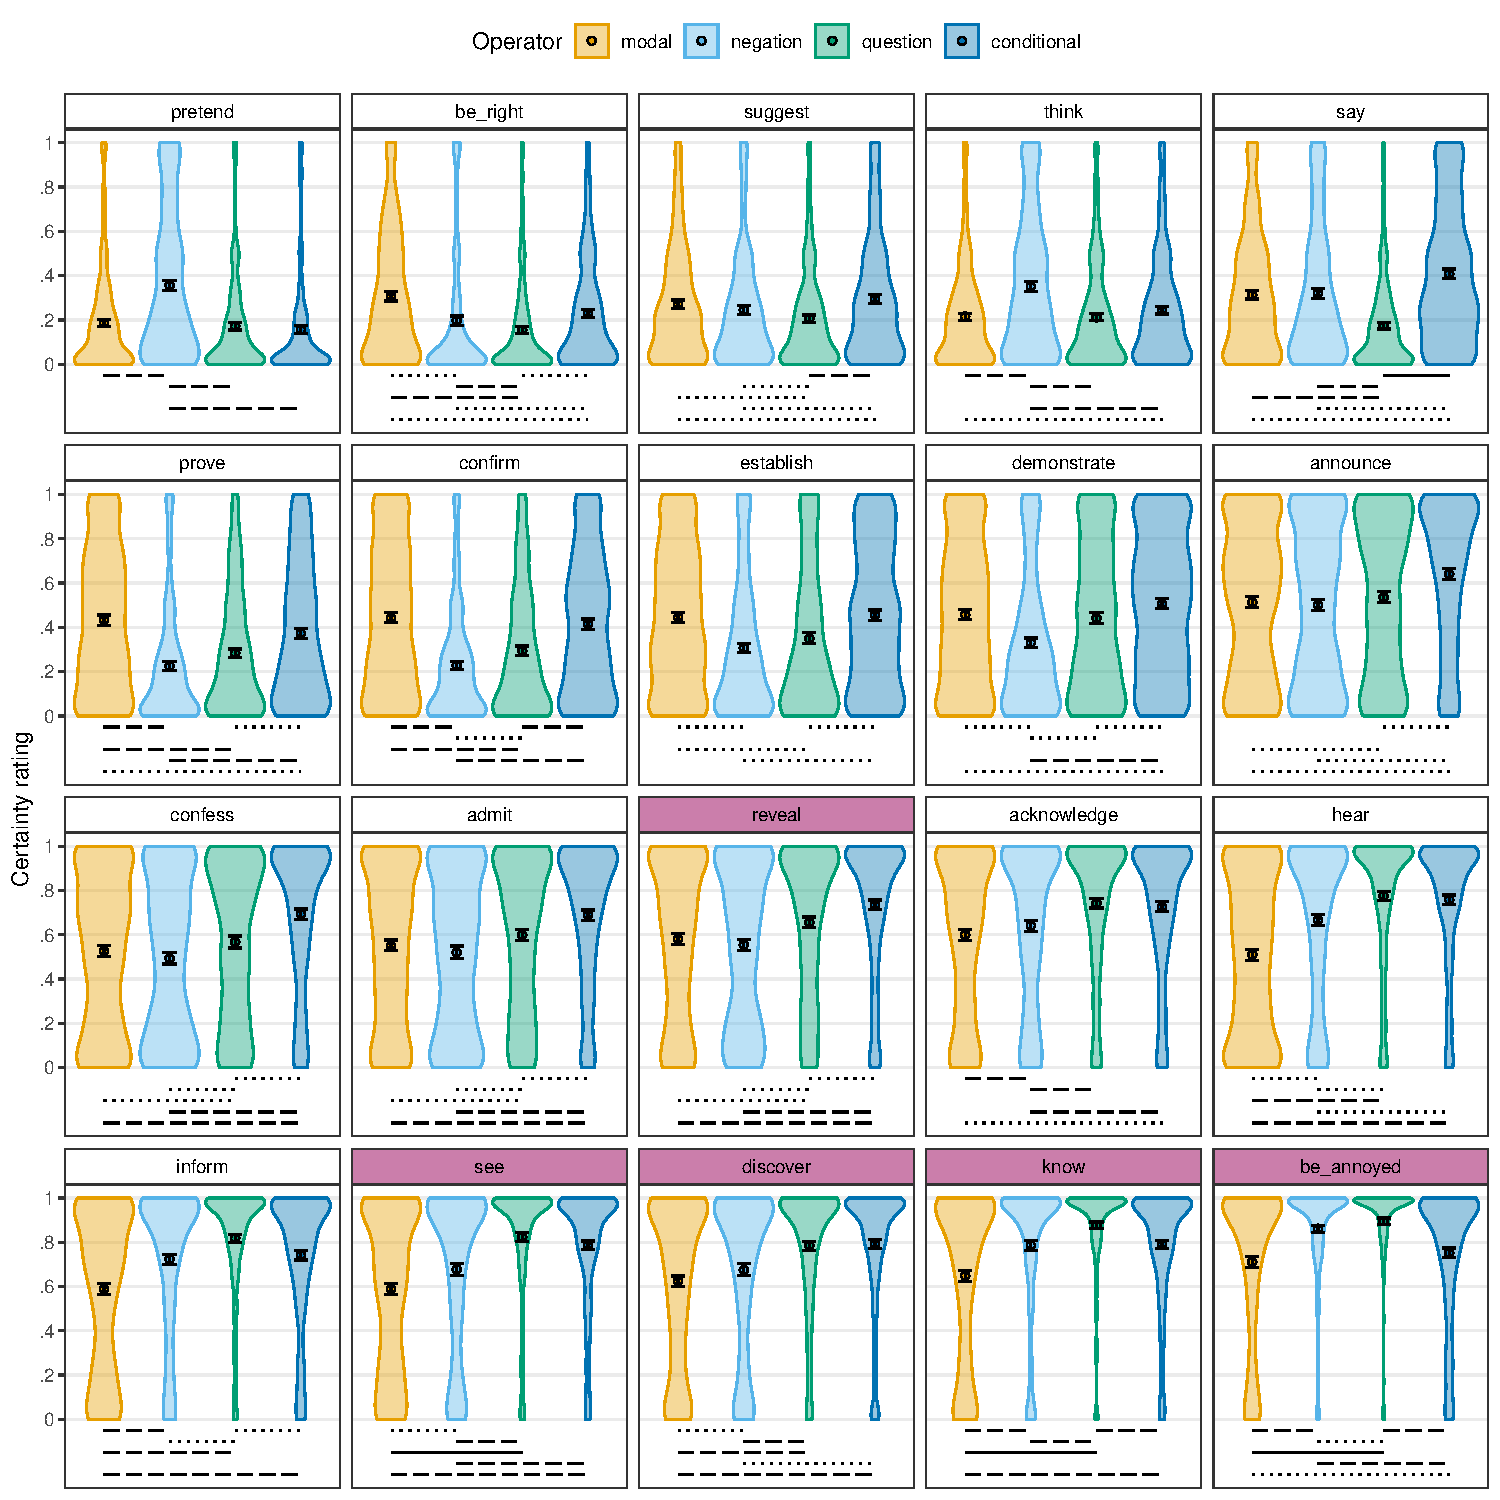
\includegraphics[width = .9\linewidth]{analysis.pdf}
    		\caption{Mean certainty ratings by predicate (\textcolor{pred-fcv-color}{(semi-)factive}, non-factive) and operator (\textcolor{op-m-color}{modal},  \textcolor{op-n-color}{negation}, \textcolor{op-q-color}{polar questions}, \textcolor{op-c-color}{conditional antecedents}) with 95\% bootstrapped confidence intervals. Violin plots indicate kernel probability density of individual participants' ratings. Predicate facets are ordered by the predicate mean certainty rating (aggregating across operators). Below each facet, a line spanning two operators indicates a non-zero difference according to the pairwise comparison of operators. The line type indicates whether the difference $d$ is $\geq 1$ (solid line: —), $0.5 \le d < 1$ (dashed line: – –), $0 \le d < 0.5$ (dotted line: . . . ).}
            %at least $1$ (solid line: —),
            %below $1$ but at least $0.5$ (dashed line: – –),
            %or below $0.5$ but above $0$ (dotted line: . . . )}
    		\label{fig:op-pred-analysis}
    	\end{figure}

        
        
    

        We also observe by-operator projection variation for non-factive predicates. Some of this variation aligns with that observed for factive predicates: For instance, the CC of \emph{inform} exhibits the same pattern as the CC of \emph{know}, and the CCs of \emph{hear} and \emph{see} the same pattern as that of \emph{discover}. Other non-factive predicates exhibit other patterns: the CCs of \emph{admit}, \emph{confess} and \emph{announce} project most from the conditional antecedents than the other three operators. 

        These observations are supported by post-hoc pairwise comparisons of the estimated means for each entailment-canceling operator within each predicate using the \texttt{emmeans} package (\citealt{emmeans}). The input to the pairwise comparisons for each predicate were 20 Bayesian mixed-effects beta regression models that were fit using the \texttt{brms} package (\citealt{buerkner2017}) with weakly informative priors. The models for each predicate predicted certainty ratings\footnote{To model the certainty ratings using a beta regression, the ratings were first transformed from the interval [0,1] to the interval (0,1) using the method proposed in \citealt{smithson_better_2006}.} from a fixed effect of entailment-canceling operator (with treatment coding and `modal' as the reference level) and included a random by-item intercept and a random slope for operator by item.\footnote{See Supplement F for further details on the models.} The output of the pairwise comparisons were 95\% highest density intervals (HDIs) of estimated marginal mean differences between each of the operators for each predicate. We assume that two operators differ in certainty ratings for a given predicate if the HDI of their pairwise comparison does not include 0. These non-zero differences between two operators are indicated by lines spanning the two operators below each predicate facet in Figure~\ref{fig:op-pred-analysis}.


        %More generally, we found by-operator differences for the CC of each of the 20 clause-embedding predicates, and that the effect of operator differs between predicates.
        %
        Our findings align with those of \citealt{smith_relationship_2014}, who also observed by-expression variation in the effect of operator. However, while they found that the CC of \emph{know} projects more from under negation than the antecedent of a conditional, we did not find a difference here. We hypothesize that this difference is due to the difference in projection diagnostic used. Our results differ, however, from those of \citealt{sieker_projective_2022}. While their work did not find differences in by-operator projection variation between factive and semi-factive predicates, our results suggest four different patterns of by-operator variation for the five (semi)factive predicates. As \citealt{sieker_projective_2022} also used the `certain that' diagnostic for projection, this difference in results is not likely due to the projection diagnostic. Other factors that varied between our experiments are the language under investigation (German vs.\ English), the clause-embedding predicates investigated, and the CCs that the predicates were paired with. Future research will need to establish which of these factors are implicated in the observed differences.
   
        %   , who found no difference between the two groups of predicates they assumed in the effect of operator.
			%
			%However in line with Sieker \& Solstad, our results question \posscite{karttunen_observations_1971} proposed difference between factive and semi-factive predicates (see also \citealt{beaver_have_2010}). Although our data replicate the result from \citet{tonhauser_how_2018} that, in polar questions, the CC of semi-factive \emph{discover} is less projective than that of \emph{know}, the same does not hold in conditionals, contrary to what would be expected based on \posscite{karttunen_observations_1971} distinction between factive and semi-factive predicates.
			%
			%Further, the CC of (factive) \emph{be annoyed} does not project invariably from all four operators, and the CC of \emph{discover,}  which is considered semi-factive, does not project more from under negation than the other three operators. The pattern observed for {\em know} does not fit into either category.

	\subsection{Factive vs.\ non-factive predicates}\label{s:factivity}

        Lexical approaches to projection assume that factive predicates are ones that presuppose the CC, while the CC of non-factive predicates is not presupposed (e.g., \citealt{kiparsky_fact_1970,karttunen_observations_1971,schlenker_local_2010,abrusan_predicting_2011}).\footnote{Some of these works additionally assume that the CC of factive predicates is entailed. For details see \citealt{degen_are_2022}.} Because presuppositions are assumed to typically project from under entailment-canceling operators, this definition predicts that factive predicates are distinguished from non-factives by the projection of their CCs: The CCs of factive predicates are expected to be categorically more projective than those of non-factives. This expectation was investigated in \citealt{degen_are_2022} based on the 20 clause-em\-bed\-ding predicates in \ref{ex:predicates} embedded in polar questions. Contrary to expectation, \poscite{degen_are_2022} Exps.~1 found that the CCs of the five (semi-)factive predicates varied in projection, that the CCs of the 15 non-factive predicates were projective compared to the non-projective main clause contents, and that the CCs of some non-factives were as projective, or even more projective, than those of some factive predicates.  In short, projection of the CC from under polar questions did not categorically distinguish factive from non-factive predicates. Further support for this result came from analyses of projection ratings in three additional datasets, namely the CommitmentBank (\citealt{de_marneffe_commitmentbank_2019}), the VerbVeridicality dataset (\citealt{ross_how_2019}), and the MegaVeridicality  dataset (\citealt{white_role_2018}).
        
        

        The results of the experiments reported on in this paper replicate \poscite{degen_are_2022} result. As shown in Figure~\ref{fig:op-pred-ratings-q}, there is variation between the five \textcolor{pred-fcv-color}{factive} predicates in the polar question condition, and projection from under polar questions does not categorically distinguish factive from non-factive predicates. Furthermore, our results suggest that this result can be extended to the three other entailment-canceling operators. As shown in Figures~\ref{fig:op-pred-ratings-m}-\ref{fig:op-pred-ratings-c}, there is variation in the projection of the CCs of the five factive predicates from under \emph{perhaps}, negation, and conditional antecedents, and projection ratings in these conditions do not show a categorical difference between factive and non-factive predicates either.  These results lend further support to the conclusion of \citealt{degen_are_2022} that there is, to date, no empirical evidence for a coherent class of factive predicates.

        %Instead, we see a gradient  effect of predicate on projection ratings in all four conditions.

        \begin{figure}[h!]
            \centering
            \begin{subfigure}[t]{0.49\textwidth}
            \caption{Polar question}
            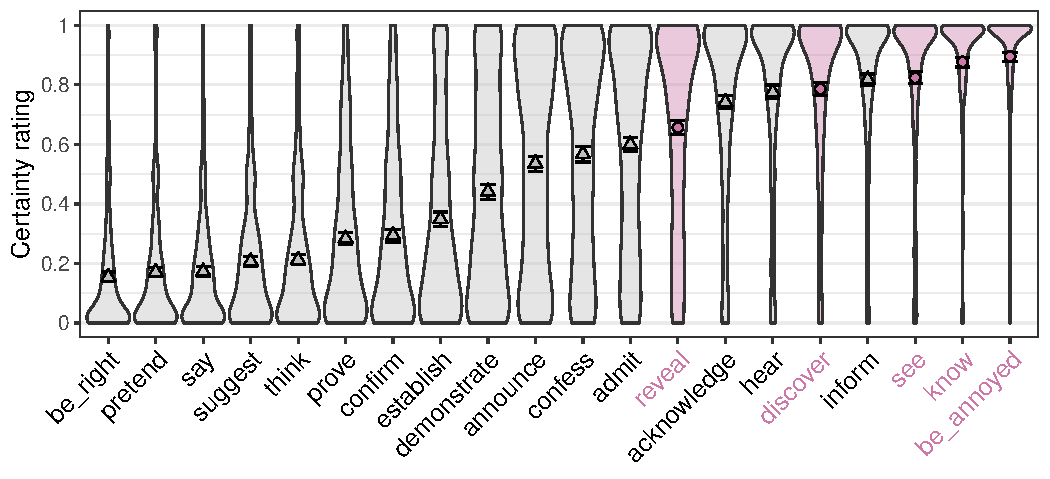
\includegraphics[width = 1\linewidth]{question-predicate-graph.pdf}
            \label{fig:op-pred-ratings-q}
            \end{subfigure}
            %
            %\vspace{-\baselineskip}
            %\medskip
            \begin{subfigure}[t]{0.49\textwidth}
            \caption{Modal \emph{perhaps}}
            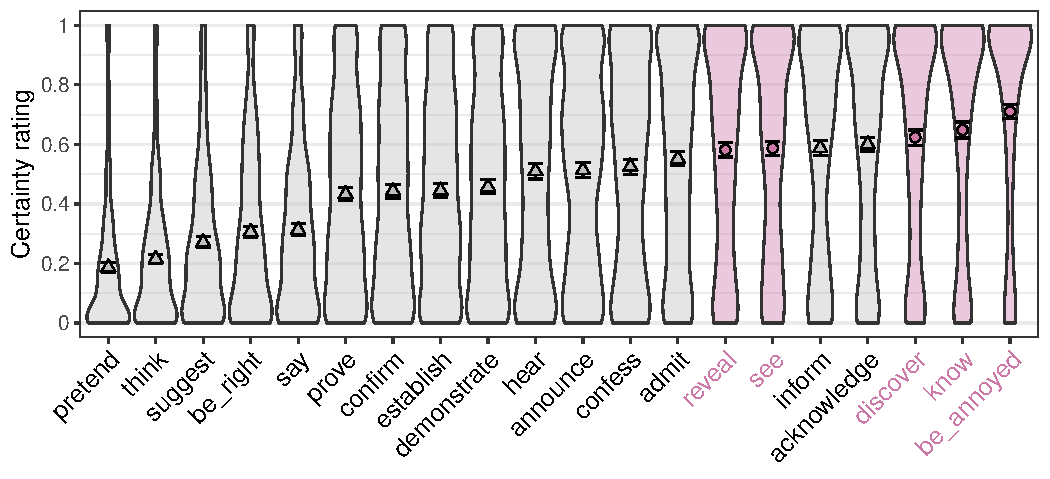
\includegraphics[width = 1\linewidth]{modal-predicate-graph.pdf}
            \label{fig:op-pred-ratings-m}
            \end{subfigure}

            \vspace{-\baselineskip}
            %\medskip
            \begin{subfigure}[t]{0.49\textwidth}
            \caption{Negation}
            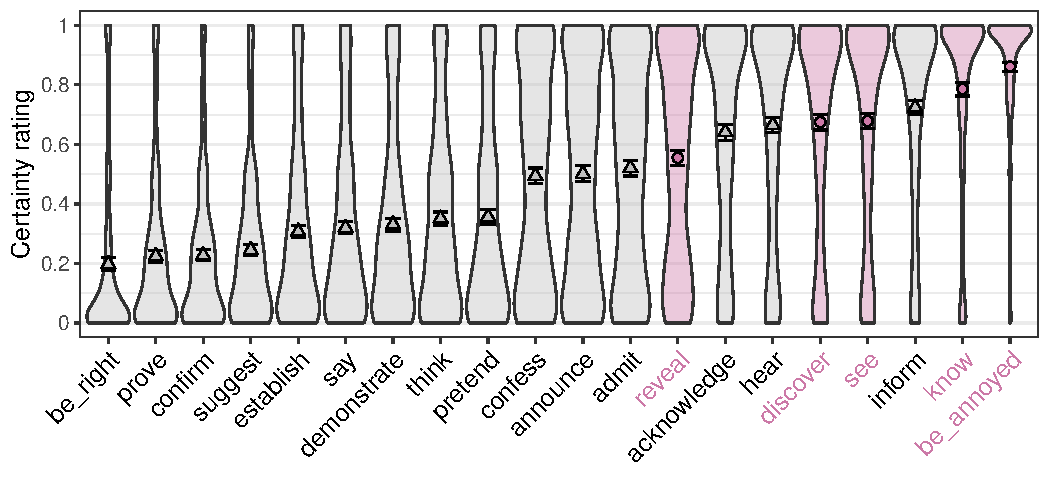
\includegraphics[width = 1\linewidth]{negation-predicate-graph.pdf}
            \label{fig:op-pred-ratings-n}
            \end{subfigure}
            %
            %\vspace{-\baselineskip}
            %\medskip
            \begin{subfigure}[t]{0.49\textwidth}
            \caption{Conditional}
            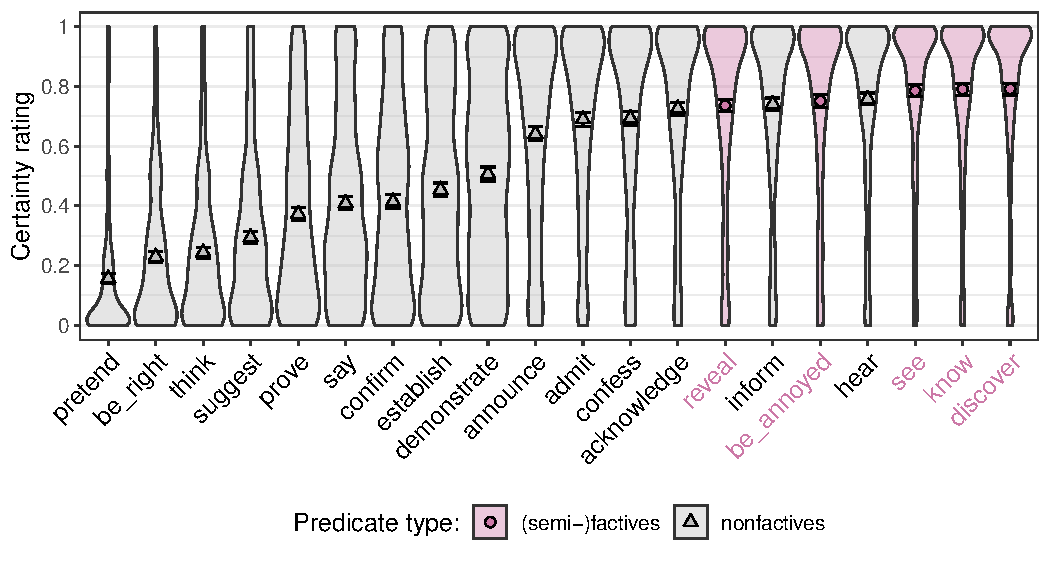
\includegraphics[width = 1\linewidth]{conditional-predicate-graph.pdf}
            \label{fig:op-pred-ratings-c}
            \end{subfigure}

            \vspace{-\baselineskip}
            \caption{Mean certainty ratings by predicate, with (semi-)factive predicates in \textcolor{pred-fcv-color}{violet}, for (a) polar questions, (b) the modal \emph{perhaps}, (c) negation, (d) conditional antecedents. Error bars indicate $95\%$ bootstrapped confidence intervals. Violin plots indicate kernel probability densities of the individual participants’ ratings.}\label{fig:op-pred-ratings2}
        \end{figure}

        % The results of the experiments reported on in this paper replicate this result. As shown in Fig.~\ref{fig:op-pred-ratings-q}, there is variation between the CCs of the five factive predicates in the polar question condition, and projection from under polar questions does not categorically distinguish factive from non-factives predicates. This result replicates the results of \poscite{degen_are_2022} Exps.~1. Furthermore, the results of the experiments reported on in section \ref{s2} suggest that projection from under the three other entailment-canceling operators also does not categorically distinguish factive and non-factives predicates. As shown in Figs.~\ref{fig:op-pred-ratings-m}-\ref{fig:op-pred-ratings-c}, there is variation in the projection of the CCs of the five factive predicates from under the other three entailment-canceling operators, and projection from under the other three entailment-canceling operators also does not categorically distinguish factive from non-factives predicates. These results strengthens the conclusion of \citealt{degen_are_2022} that there is, to date, no empirical evidence for a coherent class of factive predicates.

   
	\subsection{Summary}

        The results of our experiments suggest that there is little by-operator variation when aggregating over clause-embedding predicates, but that the CCs of different clause embedding predicates exhibit by-operator projection variation. 
        %
        Crucially, the effect of operator on projection differs by predicate, but not in ways that align with prior claims about differences between factive and semi-factive predicates (e.g., \citealt{karttunen_observations_1971}). Finally, the results of our experiments provide further support for the results of \citealt{degen_are_2022}, who did not find empirical support for a class of factive predicates based on the projection of the CC from under polar questions. Our experiments suggest that projection of the CC from under negation, the antecedent of conditionals and epistemic modals also do not provide empirical support for a natural class of factive predicates. Before discussing the methodological and theoretical implications of these results in Section~\ref{s:general}, we provide converging evidence from a different dataset in Section~\ref{s:converging}.
   
   
\section{Converging evidence for the by-predicate variation in the effect of operator}\label{s:converging}

    We provide converging evidence for the by-predicate variation in the effect of operator based on the Mega\-Ve\-ri\-dicality dataset (\citealt{white_role_2018}). This dataset contains projection ratings for the CCs of 517 English clause-embedding predicates. As shown in \Next for \emph{know}, the predicates were combined with (what the authors refer to as) ``low lexical content''. %Indeed, the stimuli that participants rated consisted of combinations of these predicates with what White and Rawlins 2018 referred to as ‘low content arguments’, as shown in \Next for \emph{know}. %The predicates were embedded under negation \Next[a], in the antecedent of a conditional and a polar question \Next[b], and under negation, in the antecedent of a conditional, and in a question \Next[c]. To assess projection, participants were asked to respond to the question \emph{did that thing happen?} %for stimuli like \Next[a] and to respond to the question posed by stimuli like \Next[b] and \Next[c].
    %The response options were ‘yes’, ‘maybe or maybe not’, and ‘no’.
    The predicates were embedded under negation as in \Next[a], in the antecedent of a conditional as in \Next[b], and under negation in the antecedent of a conditional as in \Next[c]. To assess projection, participants were asked to respond to the question \emph{did that thing happen?}.\footnote{In \ref{mvb} and \ref{mvc}, the participants responded to a question presented in the consequent of the conditional. Thus, the predicates in these two conditions may also be taken to be embedded in a polar question.} %for stimuli like \Next[a] and to respond to the question posed by stimuli like \Next[b] and \Next[c].
    The response options were ‘yes’ (indicating projection), ‘maybe or maybe not’, and ‘no’ (no projection).

	%Our experimental result that that the effect of entailment-cancelling operator differs by predicate finds further support in the data from \posscite{white_role_2018} MegaVeridicality dataset.
	%
	%White \& Rawlins assess projection inferences associated with 517 clause-embedding predicates by presenting them in 50 \lq low-content\rq\ syntactic frames, like the ones in \Next, illustrated here with \textit{know}. The frames in \Next present predicates associated with projective contents embedded under negation \Next[a], in conditional antecedents \Next[b], or both \Next[c], in combination with a projection question (\textit{Did that thing happen?}).

			\ex. \a. Somebody didn’t know that a particular thing happened. Did that thing happen?
				\b.\label{mvb} If somebody knows that a particular thing happened, did that thing happen?
				\b.\label{mvc} If somebody didn’t know that a particular thing happened, did that thing happen?
				\z.
			\z.

    To investigate by-predicate projection variation, we recoded the responses as 1 (`yes'), -1 (no), and 0 `maybe or maybe not'). We calculated the mean projection ratings for 25 predicates under the three types of operator combinations shown in \Last. We used the 14 non-factive and 5 factive predicates from our experiments that are in MegaVeridicality (\textit{be right} is not included). As \citealt{djarv_cognitive_2018} suggested that the factive/semi-factive distinction can be understood as a difference between cognitive and emotive predicates, we included the emotive (\textit{disappoint}, \textit{surprise}) and cognitive (\textit{realize}, \textit{find out}) predicates from their experiments that are in MegaVeridicality. We also added two other predicates suggested by Karttunen as factive (\textit{regret}) and semi-factive (\textit{notice}).

           	\begin{figure}
				\centering
				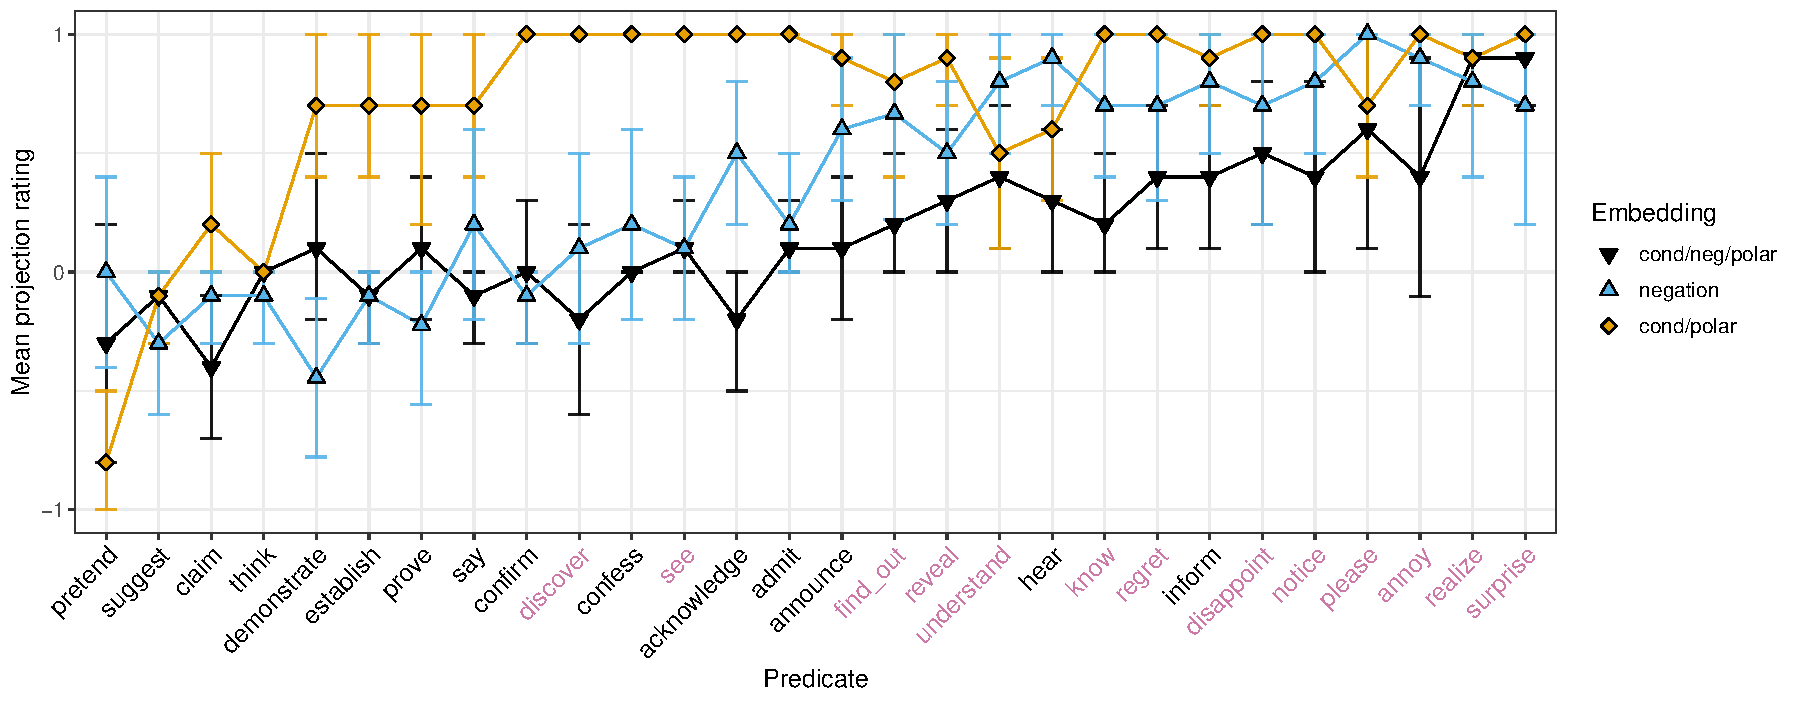
\includegraphics[width = \linewidth]{megaveridicality}
				\caption{Mean projection ratings by entailment-canceling operator(s) and clause-embedding predicate in the MegaVeridicality dataset.}
				\label{fig:megaverid}
			\end{figure}

    Figure \ref{fig:megaverid} shows mean projection ratings by embedding operator(s) and predicate. As shown, the effect of operator varies by predicate: For many predicates, ratings are (at least numerically) lower when embedded under negation, or under negation and in a conditional antecedent, than when embedded in a conditional antecedent. These observations suggest that there is by-predicate variation in the effect of entailment-canceling operator even when projection ratings are collected with a different measure and different materials than in our experiments. 

    %In a series of experiments, participants presented with stimuli like \Last responded with \lq yes\rq, \lq no\rq, or  \lq maybe\rq (coded as \texttt{1, -1,} or \texttt{0}, respectively). Here, we present data from their data set, for the frames in \Last, and 16 of their predicates. These include ones also used in our experiment as purported factives (\textit{be annoyed, know, reveal}) and semi-factives (\textit{discover, see}), and eleven further predicates commonly characterized as factive or semi-factive (\textit{amuse, find out, forget, learn, love, notice, realize, recognize, regret, remember, understand}).

	% the predicates \textit{see} and \textit{learn} have the same mean ratings for both negative and conditional contexts. However, the effect of negative conditional contexts does not simply reflect the additive result of both effects, but 

	%It is worth noting that the task assesses global projection only in case of \Last[a], but not \Last[b+c], where the question \textit{did it happen?}\ is embedded in the conditional consequent. It assesses whether the projective inference holds in the conditional local context.
 
    %Nevertheless, the data provides supporting evidence for by-predicate variation in the effect of operators on projection. %Crucially, the by-predicate variation in the effect of negation in the global context is different from the by-predicate variation in the effect of negation in the conditional context.
    %Crucially, the by-predicate variation in the effect of negation alone is different from the by-predicate variation in the effect of negation in the conditional context.


\section{General discussion}\label{s:general}

    We now point out methodological implications of our results (Section~\ref{s:method-impl}), discuss whether contemporary projection analyses can capture the observed variation (Section~\ref{s:analysis}), and speculate about lexical differences between the clause-embedding predicates that might predict the by-operator variation observed (Section~\ref{s:lex}).

\subsection{Methodological implications}\label{s:method-impl}

    The results of the experiments reported on in Section~\ref{s2} suggest that there is little by-operator projection variation when aggregating observations for the CCs of the  clause-embedding predicates, but that there is by-operator variation that cannot be neglected when we do not aggregate. These results have two methodological implications. First, when initially investigating the projection of a content (or teaching projection to students), the family-of-sentences can indeed be treated as a family, as standard textbooks assume. However, it is advisable to apply the diagnostic with all four operators and attend to possible by-operator projection variation. 

	A second methodological implication of the results of our experiments is that research on projection should take into account possible by-operator variation when choosing which entail\-ment-canceling operator to use. Further, results about projection variation should be relativized to the entailment-canceling operator under which the expressions and contents were embedded, as they may very well depend on this choice. For instance, two contents that exhibit projection variation when embedded under polar questions might not exhibit such differences with a different entailment-canceling operator, and two contents that do not exhibit projection variation from under negation might exhibit variation when embedded under some other operator.

\subsection{Theoretical implications}\label{s:analysis}

    This section discusses whether contemporary analyses can capture the observed by-predicate projection variation and the interactions between predicate and entailment-canceling operator.
	% Our results---that projection is modulated by entailment-canceling operators and that there is by-predicate variation in the effect of operator on projection---are not captured by contemporary projection analyses.

\subsubsection{\citealt{heim_projection_1983} and \citealt{van_der_sandt_presupposition_1992}}\label{s:heim}

    On the analyses in \citealt{heim_projection_1983} and \citealt{van_der_sandt_presupposition_1992}, the CCs of factive predicates are lexically specified as presupposed, in contrast to the CCs of non-factive predicates. Presupposed CCs project to the global context, except when that would produce an inconsistency, in which case they are accommodated to the local context of the operator.

    These analyses do not predict the observed by-predicate variation, for several reasons. One reason is  variation among the factive predicates: For instance, when embedded under polar questions, negation, or \emph{perhaps,} the CC of \emph{be annoyed} is more projective than that of \emph{discover}, which in turn is more projective than that of \emph{reveal}. (In conditional antecedents, the order of \emph{be annoyed} and \emph{discover} is reversed, see Figure~\ref{fig:op-pred-ratings2}.)
    %
    This variation is not predicted because the CCs of factive predicates are invariably specified as presupposed, with no mechanism to predict projection variation between factive predicates. (Recourse to local accommodation is not possible because the stimuli in our experiments were presented in minimal contexts that were not inconsistent with the CCs.)  A second reason is that the CCs of some non-factive predicates (e.g., \emph{inform, acknowledge}) are just as projective as those of some factive predicates, or even more projective. Analyses like those in \citealt{heim_projection_1983} and \citealt{van_der_sandt_presupposition_1992} fail to make predictions about the projection of the CCs of non-factive predicates. Thus, as discussed in detail in \citealt{degen_are_2022}, the factive/non-factive distinction is not sufficiently fine-grained to adequately predict the observed by-predicate projection variation.

    The analyses in \citealt{heim_projection_1983} and \citealt{van_der_sandt_presupposition_1992} also do not predict differential effects of entailment-canceling operators on projection. This is because negation and conditional antecedents are given a semantics that derives their behavior as presuppositional holes, in the sense of \citealt{karttunen_observations_1971}. For instance in \citealt{heim_projection_1983}, presupposition triggers under negation or in conditional antecedents are evaluated relative to a local context that is equal to the global context, with the consequence that presuppositions are not expected to project differently from under negation or conditional antecedents. While the analysis does not explicitly address epistemic possibility modals or polar questions, we might expect that they would be treated as presuppositional holes along the same lines, therefore also not predicting any by-operator projection variation, or by-predicate variation in the effect of entailment-canceling operators.
	%
	%Differential effects of operators on projection could conceivably be addressed in such a system by assuming that the meaning of entailment-cancelling operators systematically affects the possibility of local accommodation (e.g., by assuming that accommodation is more likely under modals than conditional antecedents). However, no such effects have been spelled out.
		
	

\subsubsection{\citealt{abrusan_predicting_2011} and \citealt*{simons_best_2017}}\label{s:abrusan}

    \citet{abrusan_predicting_2011} and \citet{simons_best_2017} do not assume that presuppositions are lexically specified. In \citealt{abrusan_predicting_2011}, a lexical entailment of a (possibly embedded) sentence is a presupposition, if it is about a time that is not the event time of the matrix predication and it is not at-issue with respect to the Question Under Discussion (QUD, see \citealt{roberts_information_2012}) addressed by the utterance. For instance, the CC of B's utterance in \ref{ent}, that Phil's ballet class is canceled, is predicted to be a presupposition (and therefore to project) because it is a lexical entailment of the modal prejacent and not at-issue with respect to A's interrogative utterance.
    
    \ex.\label{ent} Adapted from \citealt[188]{simons_best_2017} \\ Context: It's early on Saturday morning. A and B are talking about their son. 
    \a.[A:] Why is Phil up already?
    \b.[B:] Perhaps he forgot that his ballet class is canceled today. 

    In \citealt{simons_best_2017}, the CC of a clause-embedding predicate projects if it is entailed by the Current Question of the utterance (where, roughly, the Current Question is the question that is congruent with the utterance).\footnote{The Current Question is defined in \citealt[194]{simons_best_2017} as follows: ``The Current Question for an utterance is a privileged subset of the focal alternative set of the uttered sentence (given a structural analysis of that sentence, including focus marking)'' which meets the conditions that ``i) the proposition expressed is a member of the Current Question and ii) the Current Question has at least one additional member.''} In \ref{ent},  the Current Question of B's utterance might be the set of propositions \{Phil forgot that his ballet class is canceled today, Phil is aware that his ballet class is canceled today\}. If so, the Current Question entails that Phil's ballet class is canceled today, and the CC may therefore project under \poscite{simons_best_2017} analysis.
  
    Under the analyses in \citealt{abrusan_predicting_2011} and \citealt{simons_best_2017}, CCs that are entailed based on the literal content of an utterance may or may not project, depending on whether they contribute to the main point of the utterance. This opens up the possibility for projection variation among veridical predicates (including those often characterized as factive), representing an improvement compared to the lexical specification of factivity assumed in \citealt{heim_projection_1983} and \citealt{van_der_sandt_presupposition_1992}. However, these accounts still do not predict the observed by-predicate variation.
    %
    First, to make explicit predictions about the observed by-predicate variation, these types of analyses would need to make explicit assumptions about how different predicates contribute to how the question under discussion is chosen.
    %
    % The analyses in \citealt{abrusan_predicting_2011} and \citealt{simons_best_2017} do not predict the observed by-predicate variation. First, if the CCs of factive predicates are entailed, they are invariably predicted to project, and so the observed differences between the CCs of different factive predicates are not predicted.
    %
    Second, the analyses do not make systematic predictions for non-entailed CCs, and hence they do not predict that the CCs of some non-factive predicates project at least as much or even more than those of some factive predicates.

    Both of these analyses set aside the effect of entailment-canceling operators in determining the main point of an utterance. Therefore they do not make predictions about by-operator differences or by-predicate variation in the effect of entailment-canceling operators.


\subsubsection{\citealt{schlenker_triggering_2021}}

    Under the view put forward in \citealt{schlenker_triggering_2021}, the CC of a sentence $S$ like \ref{knowa}, is presupposed in a context $c$, if the CC 
    is presupposed by the sentence $S'$ under the entailment-canceling operator, that is \ref{knowb} in the local context $c'$.
    %is an epistemic precondition on the global meaning of $S$. 
    %Formally, Schlenker defines presuppositions relative to their local context (\S6.2).
    For the CC to be presupposed in \ref{knowb}, two conditions must be met %for $S'$, the prejacent of negation in \ref{knowb}:
	i) $S'$ contextually entails the CC relative to $c'$;
	and ii) If we consider ``a generic agent'' who believes the propositions in $c'$ and who has now learned about the truth of S$'$, then the probability that this generic agent already believed the CC is above a contextual threshold $\alpha$;
	more colloquially, condition ii) requires that the generic agent ``typically antecedently believes'' the CC (p.6) upon interpreting S$'$ in $c'$. Based on \citealt{heim_projection_1983} and \citealt{schlenker_local_2009}, the the local context under negation $c'$ is assumed to be identical to the global context $c$. Therefore, epistemic preconditions relative to $c'$ will also apply to the global context. Applied to \ref{know}, \poscite{schlenker_triggering_2021} analysis predicts that the CC  is presupposed if i) \ref{knowb} contextually entails that Julian dances salsa, and ii) a generic agent ``typically antecedently believes'' that Julian dances salsa upon interpreting \ref{knowb} in the contexts provided to our participants.

	\ex.\label{know} 
	\a.\label{knowa} Cole doesn't know that Julian dances salsa.
	\b.\label{knowb} Cole knows that Julian dances salsa.
	\z.

	Condition i) is met under the assumption that the CC of \ref{knowb} is an entailment. \citealt{schlenker_triggering_2021} also assumes the condition ii) is met: ``in many cases, one's knowledge of facts will precede one's knowledge of [Cole's] beliefs about them\ldots believing that [Julian dances salsa] is often an epistemic precondition for believing that'' Cole knows that Julian dances salsa (p.6). One might, however, challenge this assumption on the basis of the corpus investigation presented in \citealt{spenader_presuppositions_2002}, which showed that the CCs of the majority of the utterances of sentences with factive verbs (namely 81 out of 109) had to be accommodated (i.e., were not contextually entailed). In other words, utterances of sentences with the factive predicates investigated by \citet{spenader_presuppositions_2002}, which included \emph{know}, were ``generally used to communicate information the speaker thought was hearer-new'' (p.99). This result might therefore suggest that one cannot assume that a generic agent typically antecedently believes the CC of {\em know}.

    \poscite{schlenker_triggering_2021} analysis does not incorporate differential effects of entailment-canceling operators on projection. As discussed for \citealt{heim_projection_1983} above, the local contexts under negation and in conditional antecedents are both assumed to be the global context (and similarly in \citealt{schlenker_local_2009}). Therefore, the analysis does not make predictions about by-operator projection variation or about by-predicate variation in the effect of entailment-canceling operator.

    Does the account capture the observed by-predicate variation?
    %
    The account takes the subjective conditional probabilities associated with expressions and the contextual threshold $\alpha$ as given, and therefore does not offer explicit or systematic predictions about projection ratings for different expressions.
    %
    We, therefore, assume that it is an open, empirical question which predicates are such that the probability of a generic agent antecedently believing the CC is above the contextual threshold $\alpha$ in the minimal contexts we provided our participants (and, of course, what that threshold might be).
    
    Throughout the discussion, however, \citealt{schlenker_triggering_2021} appears to assume that there are two classes of predicates: those where the probability is usually above the threshold (including {\em know, inform}, and {\em announce}), and those where it is not (including {\em demonstrate} and {\em establish}; see p.12 and appendix I).
    %
    As this division does not fall along the lines of traditionally assumed classes of (non-)factives,
    % Thus,
    one advantage of \poscite{schlenker_triggering_2021} analysis over the analyses reviewed in Sections~\ref{s:heim} and \ref{s:abrusan} is that it predicts the projection of the CCs of (certain) non-factive predicates (modulo the open questions about condition ii).

    Based on these assumptions, the analysis correctly predicts that the CCs of \emph{know, inform}, and \emph{announce} are more projective than the CCs of \emph{demonstrate} and \emph{establish}, by virtue of the CCs of the former being usually presupposed, in contrast to the CCs of the latter. It is not clear, however, that the analysis is able to predict the observed variation, because the analysis -- even  though it does not divide predicates into factive and non-factive ones -- nevertheless imposes a binary, categorical distinction between predicates.
    % such that the CCs of predicates with probabilities that are usually above the threshold are presupposed, and those below the threshold are not.
    %
    Crucially, the by-predicate variation reported in Sections~\ref{s:by-pred} and \ref{s:factivity} is not captured by an analysis that does not make more fine-grained distinctions between the meanings of clause-embedding predicates, as discussed extensively in \citealt{degen_are_2022}. First, there is projection variation between the supposedly presupposed CCs (that of \emph{know} is more projective than the CC of \emph{inform}, which is more projective than that of \emph{announce}, under all four operators).
    %
    Furthermore, as discussed in \citealt{degen_are_2022}, the CCs of the supposedly nonpresupposed CCs (of \emph{establish} and \emph{demonstrate}) are projective when compared to nonprojective main clause content. In the experiments reported on in Section~\ref{s2}, the mean certainty rating of the CC of \emph{announce}, whose CC is assumed to possibly be presupposed, is $.55$, and that of {\em demonstrate}, whose CC is not assumed to be presupposed, is $.43$ (both means are aggregated across entailment-canceling operators). It is not clear whether this particular difference in mean certainty rating motivates analyzing the CC of \emph{announce} as presupposed in contrast to that of \emph{demonstrate}.

\subsubsection{Interim summary}

    There is currently no projection analysis on the market that predicts the by-predicate and by-operator variation we observed in the experiments from Section~\ref{s2}. \citealt{degen_are_2022} suggested that an empirically adequate analysis to capture the observed by-predicate variation requires consideration of ``more fine-grained distinctions [between clause-embedding predicates] that are based on the lexical meaning and discourse use of clause-embedding predicates'' (p.~585). Further, an account of the observed by-predicate variation in the effects of entailment-canceling operators will need to consider how semantic and pragmatic properties of predicate meanings interact with entailment-canceling operators. We offer some suggestions based on the data from our experiments in the next section.  


\subsection{Lexical patterns}\label{s:lex}

The results of our experiments suggest that there is by-predicate variation in the effect of entailment-canceling operator. In this section, we suggest that the observed variation may be predictable, at least in part, from lexical semantic and pragmatic properties shared by subsets of the 20 clause-embedding predicates featured in our experiments. Specifically, we observe that the projection of the CCs of the 20 predicates we investigated exhibit (what we call) `projection patterns', such that the CCs of several predicates exhibit the same or at least a similar by-operator projection variation. The six patterns we identified based on our results are shown in Figure~\ref{fig:patterns}, which shows mean certainty ratings for the four operators by projection pattern.
    
    %Can the observed interactions between predicate and entailment-canceling operator be predicted from lexical semantic/pragmatic properties of the predicates? This is a pressing question for future research, to which our data offer some tentative answers. 
    
    %We can find some initial generalizations over lexical properties, indicated in Figure~\ref{fig:patterns}, which gives the mean certainty ratings for the four operators by predicate, identifying six groups of predicates that show similar by-operator variation.
	
	\begin{figure}[ht]
		\centering
		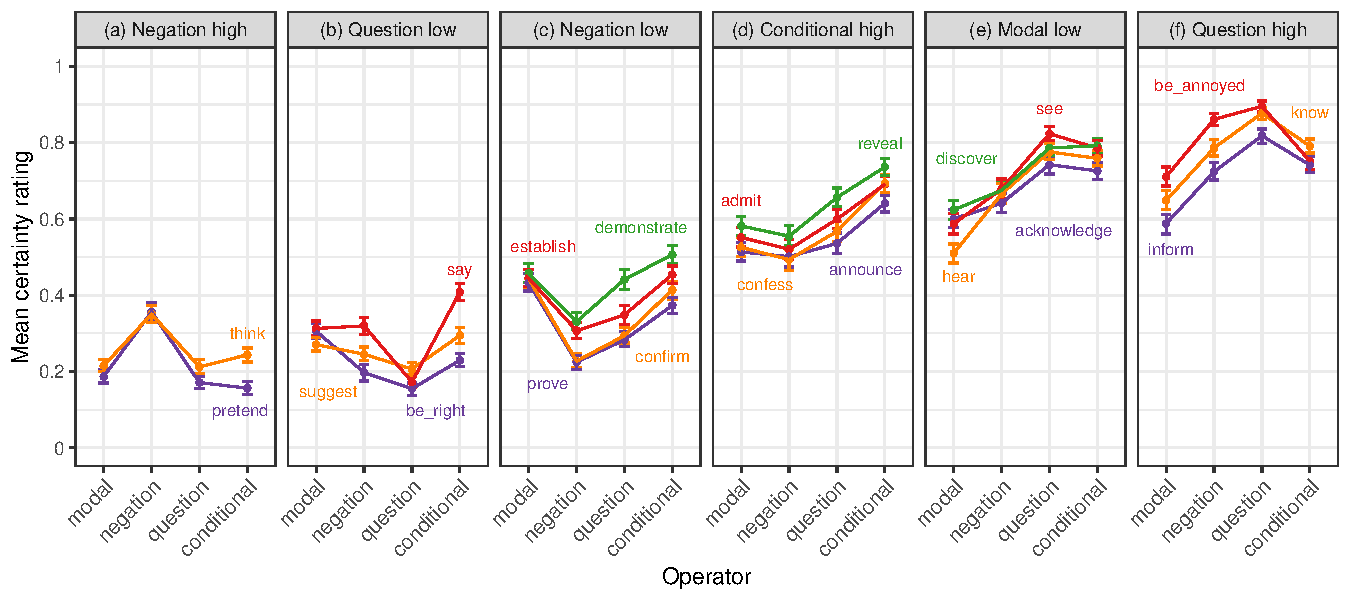
\includegraphics[width=\textwidth]{predicate-profiles.pdf}
		\caption{Mean certainty ratings by operator and predicate, by projection pattern. Error bars indicate $95\%$ bootstrapped confidence intervals.}
		\label{fig:patterns}
	\end{figure}

We suggest that these patterns are not accidental, but that the predicates that share a pattern also share lexical semantic and pragmatic meanings. For instance, the non-veridical predicates \emph{pretend} and \emph{think} exhibit the `Negation high' pattern, shown in panel (a) of Figure~\ref{fig:patterns}. These are the only predicates that are most projective under negation compared to all other operators. This generalization, supported by the statistical analysis in Section~\ref{s:by-pred} (Figure~\ref{fig:op-pred-analysis}), might be derivable from the observation that there is an anti-veridical inference for the CC of both \emph{think} and \emph{pretend}. For \emph{think}, this anti-veridical inference can arise from the fact that \emph{think} has a veridical alternative in \emph{know}  
(e.g., \citealt{heim_artikel_1991,chemla_epistemic_2008}). We tentatively hypothesize that this can lead to an inference that the CC is false in upward-monotone contexts, but not under negation. For \emph{pretend}, one might either assume a similar alternative or investigate whether this predicate entails that the speaker assumes that the CC is false. 

%assumptions that non-veridical doxastics like \emph{think} can often be interpreted in comparison to a stronger veridical alternative e.g., \citealt{heim_artikel_1991,chemla_epistemic_2008}). We tentatively hypothesize that this can lead to an inference that the CC is false in upward-monotone contexts, but not under negation. A similar alternative seems to be salient for \emph{pretend}, but not the non-veridical communicative predicates \emph{say} or \emph{suggest}.

The predicates \emph{suggest, be right}, and \emph{say} (`Question low' pattern, panel (b)) are the only predicates which are least projective in polar questions (again see Figure \ref{fig:op-pred-analysis}). We tentatively suggest that these predicates can interact with the pragmatics of polar questions in a way that can lead to an inference of incredulity towards the CC. However, there are also some differences between these predicates. The veridical \emph{be right} is most projective under modals (M $>$ C $>$ N $>$ Q), whereas \emph{say} and \emph{suggest} are most projective in conditional antecedents (C $>$ \{M,  N\} $>$ Q).

	%(c+d)
The two $\cup$-shaped patterns in panels (c) and (d) are characterized by relatively low projection ratings with negation and high ratings with conditionals. While there is fine-grained variation with regard to which the by-operator differences were statistically supported, (c) and (d) can be distinguished by their ratings for the modal. The predicates \emph{admit}, \emph{announce}, \emph{confess} and \emph{reveal}, exhibit relatively low projection ratings of the CC when embedded under \emph{perhaps} (C $>$ Q  $>$ \{M, N\}). In contrast, the predicates \emph{confirm, demonstrate, establish}, and \emph{prove} exhibit relatively high ratings with \emph{perhaps} (\emph{confirm}, \textit{prove}: M $>$ C $>$ Q $>$ N; \emph{demonstrate:} C $>$ \{M, Q\} $>$ N; \emph{establish:} \{C, M\} $>$ \{Q, N\}). For an explanation of the high conditional ratings, one might examine ways in which the discourse effect of a conditional interacts with a change-of-state meaning component of these inferential and communicative predicates. A possible explanation for the relatively low negation ratings is that these predicates can be interpreted relative to contextual assumptions that lead to a neg-raising type inference more readily than others (so that, for instance, not announcing $p$ amounts to communicating not $p$, or not proving $p$ amounts to inferring not $p$).
	
	%(e+f)
	Finally, the two $\cap$-shaped patterns in (e) and (f) are characterized by relatively high projection ratings with questions, and low ratings with {\em perhaps}. We can distinguish the two patterns by their relative ratings for conditionals. The predicates \emph{acknowledge, discover, hear,} and \emph{see}, which are associated with a change of some informational state, show relatively high ratings with conditionals (\{Q, C\} $>$ N $>$ M). The ratings for conditionals are relatively lower for the predicates \emph{be annoyed} (Q $>$ N $>$ C $>$ M), and \emph{inform}, and \emph{know} (Q $>$ \{N, C\} $>$ M), whose CCs are among the most projective.

    Although the patterns we have identified here are tentative and only based on few predicates, we believe that future investigations into shared projection patterns across a wider range of predicates is a fruitful enterprise for future investigations of projection inferences.

\section{Conclusion}

This paper investigated variation in projection from under the four entailment-canceling operators that have traditionally been used in the family-of-sentences diagnostic for projection, namely negation, polar questions, epistemic modals, and conditional antecedents. The results of our experiments suggest that the projection of the contents of the clausal complements of clause-embedding predicates varies across these operators. As discussed, there is currently no projection analysis on the market that is able to predict the observed by-predicate variation or the by-operator variation. The results of our experiments also extend a result of \citealt{degen_are_2022}, that projection ratings in polar questions do not categorically distinguish factive from non-factive predicates, to cases with negation, the epistemic possibility modal \textit{perhaps}, and conditional antecedents. This results strengthens the conclusion of \citealt{degen_are_2022} that there is, to date, no empirical evidence for a coherent class of factive predicates.

\bibliographystyle{sub-chicago}
\bibliography{projection}

\end{document}

\newpage
\appendix

\section{20 clauses}\label{app:a-clauses}
    The contents of the following 20 clauses, which realized the complements of the 20 clause-embedding predicates, were investigated in Exps.~1-4:

    %\begin{multicols}{2}
    \begin{enumerate}%[leftmargin=3ex,itemsep=-2pt]
        \item Mary is pregnant.
        \item Josie went on vacation to France.
        \item Emma studied on Saturday morning.
        \item Olivia sleeps until noon.
        \item Sophia got a tattoo.
        \item Mia drank 2 cocktails last night.
        \item Isabella ate a steak on Sunday.
        \item  Emily bought a car yesterday.
        \item  Grace visited her sister.
        \item Zoe calculated the tip.

    %\columnbreak
        
        \item  Danny ate the last cupcake.
        \item  Frank got a cat.
        \item  Jackson ran 10 miles.
        \item  Jayden rented a car.
        \item  Tony had a drink last night.
        \item  Josh learned to ride a bike yesterday.
        \item  Owen shoveled snow last winter.
        \item  Julian dances salsa.
        \item  Jon walks to work.
        \item  Charley speaks Spanish.
            
    \end{enumerate}
    %\end{multicols}

\section{Consequents for conditional target stimuli in Exps.~4} \label{app:b-consequents}
    We created 20 consequent clauses for the three experiments in which the 20 clauses were embedded in the antecedent of a conditional (Exps.~4). Each of the 20 clauses was paired with a unique consequent clause, as shown in the list below. To minimize the variation of the effect of the contents of these consequent clauses on the projection of the contents of the 20 complement clauses, the consequent clauses all consist of a uniquely named subject and an adjectival predication in the future tense ({\em will be}), and the adjectives all denote an emotion. We selected the 20 emotion-denoting adjectives based on the valence and arousal values reported in \citealt{warriner_norms_2013}: 10 of the adjectives had a positive valence, and 10 had a negative valence; all 20 adjective had an arousal value between 4.7 and 6.5. 
    
    \begin{enumerate}%[leftmargin=3ex,itemsep=-2pt]
    
    \item \ldots that Mary is pregnant, Esther will be mad.
    \item \ldots that Josie went on vacation to France, Arnold will be frustrated.
    \item \ldots that Emma studied on Saturday morning, Liam will be proud.
    \item \ldots that Olivia sleeps until noon, Elijah will be embarrassed.
    \item \ldots that Sophia got a tattoo, Ariel will be giddy.
    \item \ldots that Mia drank 2 cocktails last night, Mariela will be worried.
    \item \ldots that Isabella ate a steak on Sunday, Liz will be delighted.
    \item  \ldots that Emily bought a car yesterday, Kate will be excited.
    \item \ldots that  Grace visited her sister, Henry will be surprised.
    \item \ldots that Zoe calculated the tip, Alex will be astonished.
    \item  \ldots that Danny ate the last cupcake, Harper will be disgusted.
    \item  \ldots that Frank got a cat, Lucas will be grouchy.
    \item  \ldots that Jackson ran 10 miles, Kayla will be cheerful.
    \item  \ldots that Jayden rented a car, Brittany will be furious.
    \item  \ldots that Tony had a drink last night, Victoria will be ashamed.
    \item  \ldots that Josh learned to ride a bike yesterday, Mason will be envious.
    \item  \ldots that Owen shoveled snow last winter, Bianca will be jealous.
    \item  \ldots that Julian dances salsa, Logan will be joyful.
    \item  \ldots that Jon walks to work, Caleb will be suspicious.
    \item  \ldots that Charley speaks Spanish, Jay will be happy.
    
    \end{enumerate}

\section{Control stimuli in Exps.~1-3}\label{app:c-control}

    The control stimuli in Exps.~1-3 were the contents of main clauses. In Exps.~1q, 2q and 3q, the control stimuli consisted of the polar questions in (1). The non-restrictive relative clauses (NRRCs), given in parentheses in (1), were included in Exps.~2q and 3q, where at-issueness was measured with an assent diagnostic. The control stimuli here consisted of two clauses (like the target stimuli), to allow the relevant speaker to assent with one of two clauses.

    \ex.[(1)] Sentences for control stimuli in in question embedding experiments (Exps.~1q, 2q and 3q)
      \a. Do these muffins (, which are really delicious,) have blueberries in them?
      \b. Does this pizza (, which I just made from scratch,) have mushrooms on it? 
      \b. Was Jack (, who is my long-time neighbor,) playing outside with the kids? 
      \b. Does Ann (, who is a local performer,) dance ballet?
      \b. Were John's kids (, who are very well-behaved,) in the garage?
      \b. Does Samantha (, who is really into fashion,) have a new hat?
      \z.
    \z.

    We expected participants to give low responses on the `certain that' diagnostic for the control stimuli in (1), indicating that the speaker is not certain of the main clause content, because main clause content is hypothesized to not project out of polar questions. These expectations were borne out, as shown in the third column of Table~\ref{t-controls} for Exps.~1q, 2q, and 3q. We also expected participants to give low responses on the at-issueness diagnostics for the control stimuli in (1), indicating that the main clause content is at-issue. These expectations were borne out for Exps.~1q and 2q, as shown in the fourth column of Table~\ref{t-controls}, but the ratings were higher than expected for Exp.~3q. See below for discussion.

    In the remaining experiments, the control stimuli consisted of the positive declarative variants of (1) given in (2). The NRRCs in parentheses were realized in Exps.~2 and 3 for the reason explained above, as well as in Exp.~1c, to make the control stimuli more similar to the target stimuli (which also consisted of two clauses, namely the antecedent and the consequent).

    \ex.[(2)]  Sentences for control stimuli in negation, modal and conditional embeddings
      \a. These muffins (, which are really delicious,) have blueberries in them.
      \b. This pizza (, which I just made from scratch,) has mushrooms on it. 
      \b. Jack (, who is my long-time neighbor,) was playing outside with the kids. 
      \b. Ann (, who is a local performer,) dances ballet.
      \b. John's kids (, who are very well-behaved,) were in the garage.
      \b. Samantha (, who is really into fashion,) has a new hat.
      \z.
    \z.

    We expected participants to give high responses on the `certain that' diagnostic for the control stimuli in (2), indicating that the speaker is certain of the main clause content, because speakers are hypothesized to be committed to the asserted main clause content. These expectations were borne out, as shown in the third column of Table~\ref{t-controls} for the `n', `m' and `c' variants of Exps.~1, 2, and 3. We expected participants to give low responses on the at-issueness diagnostics for the control stimuli in (2), indicating that the main clause content is at-issue. These expectations were borne out for the `n', `m', and `c' variants of Exps.~1, as shown in the fourth column of Table~\ref{t-controls}, but not for the `n', `m', and `c' variants of Exps.~2 and 3. See below for discussion.

    \begin{table}[h!]
        \centering
        \begin{tabular}{r r r r l }
            & &  \multicolumn{2}{c}{Mean ratings} &  \\ 
            Exp. & Control stimuli & Certainty & Not-at-issueness & At-issueness measure \\ 
            \hline
            1q & (1) & .14 & .05  & asking whether $c$ \\
            1n & (2) &  .95 & .04 & sure that $c$\\
            1m & (2) & .96 & .03 & sure that $c$\\
            1c & (2) with NRRC & .94  & .08 & sure that $c$\\
            \hline
            2q & (1) with NRRC & .18 & .07 & {\em yes}, $c$\\
            2n & (2) with NRRC& .96 & .22 & {\em yes, that's true}, $c$\\
            2m & (2) with NRRC& .96 & .25 & {\em yes, that's true}, $c$\\
            2c & (2) with NRRC& .96 & .22 & {\em yes, that's true}, $c$\\
            \hline
            3q & (1) with NRRC & .17 &  .28 & {\em yes}, but $\neg c'$\\
            3n & (2) with NRRC & .94 & .44 & {\em yes, that's true}, but $\neg c'$\\
            3m & (2) with NRRC & .93 & .50 & {\em yes, that's true}, but $\neg c'$\\
            3c & (2) with NRRC & .93 & .53 & {\em yes, that's true}, but $\neg c'$\\
            \hline
        \end{tabular}
        \caption{Mean certainty and at-issueness ratings for control stimuli, for self-declared American English participants}\label{t-controls}
    \end{table}

    As mentioned above, the mean at-issueness ratings were higher than expected in the `n', `m', and `c' variants of Exps.~2 and all four of the Exps.~3. We discuss these exceptions in more detail here because they allow us to further understand the various measures for at-issueness investigated in this paper. The example in (3a) illustrates the version of the assent diagnostic applied in Exps.~2n, 2m, and 2c: the assent particle {\em yes} is followed by the clause whose content is diagnosed, here, the content of the main clause. The related affirmation diagnostic applied in Exp.~2q (where the mean at-issueness rating was as low as expected) is illustrated in (3b).

    \ex.[(3)]
        \a. Sample control stimulus in Exps.~2n, 2m, and 2c
            \a.[A:] These muffins, which are really delicious, have blueberries in them.
            \b.[B:] Yes, that's true, they have blueberries in them.
            \z.
        Question to participants: Does A's response to B sound good?
        \b. Sample control stimulus in Exp.~2q
            \a.[A:] Do these muffins, which are really delicious, have blueberries in them?
            \b.[B:] Yes, they have blueberries in them.
            \z.
        Question to participants: Does A's response to B sound good?
        \z.
    \z.

    As shown in Table \ref{t-controls},  the group mean on the control stimuli is numerically higher (at .22 or .25) than for Exp.~2q (.07). We hypothesize that a possible explanation for this difference is that participants take A to assert both the content of the main clause and of the NRRC in (3a) but is only asking about the main clause content in (3b). Whereas B's affirmation in (3b) specifies the one content that is affirmed, B's assent in (3a) specifies only one of the two contents that A asserted, seemingly leaving out a specification of the second content, that of the NRRC. Participants may judge B's response in (3b) to be less acceptable than in (3a) because of this missing content specification. This hypothesis is consistent with the results of \posscite{syrett_experimental_2015} Exp.~3, which suggests that content of a sentence-medial NRRCs can be the target of a direct denial, though the main clause content is preferred as the target of such a denial. That the group means on the control stimuli in our Exps.~2n, 2m, and 2c are still relatively low may be due to the fact that the one content that was specified is the at-issue main clause content. One would expect lower acceptability ratings in a version of this diagnostic in which the one content that was specified is the NRRC.

    The mean at-issueness ratings for the control stimuli were also higher than expected in Exps.~3. The examples in (4) illustrate the versions of the affirmation and assent diagnostics used in these experiments:

    \ex.[(4)]
        \a. Sample control stimulus in Exp.~3q
            \a.[A:] Do these muffins, which are really delicious, have blueberries in them?
            \b.[B:] Yes, but they aren't really delicious.
            \z.
        Question to participants: Does A's response to B sound good?
        \b. Sample control stimulus in Exps.~3n, 3m, and 3c
            \a.[A:] These muffins, which are really delicious, have blueberries in them.
            \b.[B:] Yes, that's true, they but they aren't really delicious.
            \z.
        Question to participants: Does A's response to B sound good?
        \z.
    \z.

    The mean at-issueness rating for the control stimuli in Exp.~3q was comparatively higher (at .28) than for Exp.~1q (.05) or Exp.~2q (.07). We hypothesize that that this difference (especially to Exp.~2q) is due the content of the NRRC being directly denied, even though it was presented as backgrounded content in A's question (as shown in (2), the content of none of the other NRRCs was a matter of personal taste).

    The mean at-issueness ratings for the control stimuli in Exps.~3n, 3m, and 3c were numerically even higher than for Exp.~3q and, in fact, the highest across all 12 experiments (at .44, .50, and .53, respectively). There are two factors that could be implicated in the difference between Exp.~3q and Exps.~3n, 3m, and 3c: first, the NRRC is included in a polar question in the former but a declarative assertion in the latter; second, B utters an affirmation {\em yes} in the former but an assent {\em yes, that's true} in the latter. For instance, participants might judge B's direct denial of the content of the NRRC as less acceptable when A uttered a declarative assertion and B assented with that assertion using {\em yes, that's true} than when A uttered a polar question and B responded in the affirmative with {\em yes}. Both factors must be considered in future research on at-issueness measures.

\section{Participant information and data exclusion criteria}\label{app:d-participants}

    This supplement provides information on the participants of the 12 experiments and the criteria by which participants' data were excluded. The first three columns of Table \ref{t:exclusion} show, for each of the 12 experiments how many participants were recruited, their age range and mean age, and their self-reported gender; no gender data was collected in Exp.~1q. The next three columns provide information on the number of participants whose data were excluded based on the following criteria:
    
    \begin{itemize}%[itemsep=-2pt]
        
        \item `multiple': Due to an experimental glitch, some participants participated more than once in Exp.~1q. Since no information was available on which one was their first take, those participants' data was removed. 
        
        \item `language': Participants' data were excluded if they did not self-identify as native speakers of American English.
        
        \item `controls': Participants' data were excluded if their mean rating on the 6 main clause control items in the projection block was more than 2 sd above the group mean (in Exps.~1q, 2q, and 3q) or more than 2 sd below the group mean (in the remaining experiments). Participants' data were also excluded if their mean rating on the 6 main clause control items in the at-issueness block was more than 2 sd above the group mean (across all experiments).
         
        \item `variance': Participants' data were excluded if they always selected roughly the same point on the response scale for the target stimuli. To identify such participants, we first identified participants whose mean variance on the target stimuli was more than 2 sd below the group mean variance and then manually inspecting their response patterns. The data of participants who used the full scale was not excluded. 
        
    \end{itemize}

    The remaining columns of Table \ref{t:exclusion} provide information on the remaining participants, that is, the participants' data that entered into the analysis. Participants took around 9-11 minutes to complete the various experiments. Participants were paid more in Exps.~1c, 2c, and 3c than the remaining experiments because the target stimuli in those experiments were longer (as they consisted of conditionals). More women than men were recruited in many of the experiments because the experiments were run at a time when Prolific went viral on TikTok, resulting in a large number of young women registering for the service (around July 24, 2021; see \url{https://blog.prolific.co/we-recently-went-viral-on-tiktok-heres-what-we-learned/}, \\ last accessed February 4, 2022).  

    \begin{sidewaystable}[h!]
      \centering
      \begin{tabular}{l | r r r | r r r r | r r r | r }
      &  \multicolumn{3}{c|}{Recruited participants} & \multicolumn{4}{c|}{Exclusion criteria} & \multicolumn{3}{c|}{Remaining participants} &  \\ 
      Exp. & total & ages (mean) & gender (f/m/o/u) & multiple & language & controls & variance & total & ages (mean) & gender (f/m/o/u) & payment   \\ 
      \hline
      1q & 300  & 19-74 (38.2)  & --  & 5  & 7  & 35  & 0  & 242   & 21-74 (39.2) &  -- & \$1.70\\
      1n & 300  & 18-74 (33.2)  &  150/145/5/0 & 0  & 8 & 17 & 1 & 274  & 18-74 (33.3) & 141/128/5/0 & \$1.70\\
      1m & 300  & 18-74 (32.7) & 150/141/7/2  &  0 & 0  & 19 & 0   & 281   & 18-74 (32.7) & 144/129/7/1 & \$1.70 \\
      1c &  300 & 18-58 (25.9)  & 249/45/6/0 & 0 & 6  & 26 & 2  & 266  &  18-58 (24.8) & 235/25/6/0  & \$2.15 \\
      2q & 250  &  18-58 (25.5) &  201/43/6/0  & 0 & 4  & 24  & 1 & 220  & 18-58 (24.8)  & 187/28/5/0  & \$1.70 \\
      2n & 250  &  18-69 (33.2)  &  127/114/6/1 & 1  & 4  & 29 & 0& 215  &  18-69 (33.1) & 113/95/6/1    & \$1.70\\
      2m & 251  & 18-74 (31.7)  & 132/113/6/0  & 0  & 4  & 27 &  0 & 220  & 18-70 (31.9) & 116/98/6/0 & \$1.70\\
      2c &  250 &  18-56 (24.5)  & 212/30/8/0  & 0  & 0  & 26 & 0  & 224  & 18-56 (24.4) & 195/24/5/0 & \$2.15\\
      3q & 250  &  18-66 (32.4) &  140/102/7/1 &  0 & 4  & 20  & 0  &  225 & 18-66 (32.6) & 125/93//7/0  & \$1.70 \\
      3n & 250  &  18-70 (24.6) & 114/31/5/0  & 0  & 5  &  13 & 4  & 228  & 18-70 (24.3) &  198/25/5/0 &\$1.70 \\
      3m & 250  & 18-63 (25.5)  & 205/40/5/0 &  0 & 3  & 14 &  0 & 233  &  18-63 (24.8) & 197/31/5/0 &\$1.70 \\
      3c & 250  & 18-59  (27.5) & 182/64/4/0  & 0  & 3  & 17 & 0 & 230  &  18-59 (26.7)  & 177/49/4/0  & \$2.15\\
      \end{tabular}
      \caption{Recruited participants, excluded data, and remaining participants in Exps.~1, 2 and 3. Gender distinctions were `f' = female, `m' = male, `o' = other, and `u' = undeclared.}\label{t:exclusion}
    \end{sidewaystable}

\section{Analysis 1 --- Estimating operator effects on projection} \label{app:analysis-1}
    Models: Bayesian mixed effects beta regression, with:
    \begin{itemize}
        \item \textbf{Repsonse variable:} projection ratings scaled for beta-regression to transform from closed unit interval $[0,1]$ to open unit interval $(0,1)$,  using method used in \cite{degen_are_2022}, from \cite{smithson_better_2006}, for proportional data.
            $$y' = \frac{y * (n - 1) + 0.5}{n}$$
        
        \item \noindent\textbf{Fixed effect:} operator (modal, negation, question, conditional; with reference level: modal)
        
        \item \textbf{Random effects:} Predicate random intercepts

        \item Assuming a beta-distributed response variable, these effects were estimated for the mean ($\mu$) and precision ($\phi$) parameters of the beta-distribution.
        
    \end{itemize}

    \noindent The model was fit using \texttt{brms}
    % (\citealt{burkner_brms_2017}) in R (\citealt{r_core_team_r_2014}), 
    using low-information priors (\texttt{brms} defaults). The estimation used $4$ chains, $3,000$ iterations per chain, $500$ warm-up, total $10,000$ iterations saved. An excerpt from the model output is shown below, providing parameter estimates, and $95\%$ credible intervals (CIs) for the fixed effects.
     
    \begin{longtable}{lrrr}
 contrast & .value & .lower & .upper \\ 
 acknowledge - admit & -0.15 & -0.33 & 0.04 \\ 
  acknowledge - again & 1.51 & 1.27 & 1.75 \\ 
  acknowledge - also & 1.60 & 1.37 & 1.85 \\ 
  acknowledge - announce & -0.48 & -0.69 & -0.29 \\ 
  acknowledge - be annoyed & 1.31 & 1.11 & 1.53 \\ 
  acknowledge - be right & -0.43 & -0.62 & -0.23 \\ 
  acknowledge - cleft & 0.74 & 0.51 & 0.97 \\ 
  acknowledge - confess & -0.10 & -0.29 & 0.09 \\ 
  acknowledge - confirm & -0.79 & -0.99 & -0.59 \\ 
  acknowledge - demonstrate & 0.12 & -0.07 & 0.31 \\ 
  acknowledge - discover & -0.01 & -0.20 & 0.19 \\ 
  acknowledge - establish & -0.52 & -0.71 & -0.33 \\ 
  acknowledge - hear & -0.31 & -0.52 & -0.10 \\ 
  acknowledge - inform & 0.05 & -0.14 & 0.24 \\ 
  acknowledge - know & 0.56 & 0.35 & 0.77 \\ 
  acknowledge - pretend & 0.08 & -0.11 & 0.28 \\ 
  acknowledge - prove & -0.21 & -0.41 & -0.03 \\ 
  acknowledge - reveal & -0.29 & -0.47 & -0.09 \\ 
  acknowledge - say & -1.04 & -1.23 & -0.82 \\ 
  acknowledge - see & -0.08 & -0.29 & 0.12 \\ 
  acknowledge - stop & 1.33 & 1.08 & 1.56 \\ 
  acknowledge - suggest & -0.86 & -1.06 & -0.66 \\ 
  acknowledge - think & -0.96 & -1.17 & -0.75 \\ 
  acknowledge - too & 1.69 & 1.43 & 1.92 \\ 
  admit - again & 1.66 & 1.43 & 1.90 \\ 
  admit - also & 1.75 & 1.51 & 1.98 \\ 
  admit - announce & -0.34 & -0.53 & -0.15 \\ 
  admit - be annoyed & 1.46 & 1.25 & 1.65 \\ 
  admit - be right & -0.28 & -0.48 & -0.10 \\ 
  admit - cleft & 0.89 & 0.65 & 1.10 \\ 
  admit - confess & 0.04 & -0.14 & 0.23 \\ 
  admit - confirm & -0.65 & -0.85 & -0.47 \\ 
  admit - demonstrate & 0.27 & 0.08 & 0.45 \\ 
  admit - discover & 0.13 & -0.05 & 0.32 \\ 
  admit - establish & -0.37 & -0.55 & -0.19 \\ 
  admit - hear & -0.16 & -0.36 & 0.03 \\ 
  admit - inform & 0.20 & 0.01 & 0.38 \\ 
  admit - know & 0.70 & 0.49 & 0.90 \\ 
  admit - pretend & 0.22 & 0.03 & 0.41 \\ 
  admit - prove & -0.06 & -0.25 & 0.11 \\ 
  admit - reveal & -0.14 & -0.33 & 0.04 \\ 
  admit - say & -0.89 & -1.10 & -0.70 \\ 
  admit - see & 0.06 & -0.13 & 0.26 \\ 
  admit - stop & 1.47 & 1.24 & 1.70 \\ 
  admit - suggest & -0.72 & -0.92 & -0.53 \\ 
  admit - think & -0.81 & -1.01 & -0.62 \\ 
  admit - too & 1.83 & 1.60 & 2.07 \\ 
  again - also & 0.09 & -0.09 & 0.27 \\ 
  again - announce & -2.00 & -2.24 & -1.76 \\ 
  again - be annoyed & -0.20 & -0.45 & 0.05 \\ 
  again - be right & -1.94 & -2.18 & -1.70 \\ 
  again - cleft & -0.77 & -0.95 & -0.60 \\ 
  again - confess & -1.61 & -1.86 & -1.38 \\ 
  again - confirm & -2.31 & -2.55 & -2.06 \\ 
  again - demonstrate & -1.39 & -1.63 & -1.15 \\ 
  again - discover & -1.52 & -1.77 & -1.28 \\ 
  again - establish & -2.03 & -2.27 & -1.79 \\ 
  again - hear & -1.82 & -2.08 & -1.58 \\ 
  again - inform & -1.46 & -1.70 & -1.21 \\ 
  again - know & -0.95 & -1.20 & -0.70 \\ 
  again - pretend & -1.43 & -1.67 & -1.18 \\ 
  again - prove & -1.72 & -1.96 & -1.49 \\ 
  again - reveal & -1.80 & -2.04 & -1.56 \\ 
  again - say & -2.55 & -2.81 & -2.30 \\ 
  again - see & -1.60 & -1.85 & -1.35 \\ 
  again - stop & -0.18 & -0.35 & -0.01 \\ 
  again - suggest & -2.37 & -2.62 & -2.13 \\ 
  again - think & -2.47 & -2.74 & -2.22 \\ 
  again - too & 0.17 & -0.01 & 0.35 \\ 
  also - announce & -2.09 & -2.33 & -1.85 \\ 
  also - be annoyed & -0.29 & -0.55 & -0.05 \\ 
  also - be right & -2.03 & -2.27 & -1.77 \\ 
  also - cleft & -0.86 & -1.03 & -0.68 \\ 
  also - confess & -1.70 & -1.95 & -1.47 \\ 
  also - confirm & -2.40 & -2.64 & -2.16 \\ 
  also - demonstrate & -1.48 & -1.71 & -1.23 \\ 
  also - discover & -1.61 & -1.86 & -1.37 \\ 
  also - establish & -2.12 & -2.36 & -1.88 \\ 
  also - hear & -1.91 & -2.16 & -1.65 \\ 
  also - inform & -1.55 & -1.79 & -1.30 \\ 
  also - know & -1.04 & -1.29 & -0.79 \\ 
  also - pretend & -1.52 & -1.77 & -1.28 \\ 
  also - prove & -1.81 & -2.05 & -1.58 \\ 
  also - reveal & -1.89 & -2.13 & -1.65 \\ 
  also - say & -2.64 & -2.89 & -2.38 \\ 
  also - see & -1.69 & -1.93 & -1.43 \\ 
  also - stop & -0.27 & -0.45 & -0.10 \\ 
  also - suggest & -2.46 & -2.72 & -2.22 \\ 
  also - think & -2.56 & -2.81 & -2.30 \\ 
  also - too & 0.08 & -0.10 & 0.26 \\ 
  announce - be annoyed & 1.80 & 1.59 & 2.01 \\ 
  announce - be right & 0.06 & -0.14 & 0.26 \\ 
  announce - cleft & 1.23 & 1.01 & 1.48 \\ 
  announce - confess & 0.38 & 0.20 & 0.58 \\ 
  announce - confirm & -0.31 & -0.52 & -0.12 \\ 
  announce - demonstrate & 0.61 & 0.42 & 0.80 \\ 
  announce - discover & 0.47 & 0.27 & 0.66 \\ 
  announce - establish & -0.03 & -0.23 & 0.16 \\ 
  announce - hear & 0.18 & -0.03 & 0.38 \\ 
  announce - inform & 0.54 & 0.34 & 0.73 \\ 
  announce - know & 1.04 & 0.84 & 1.25 \\ 
  announce - pretend & 0.56 & 0.36 & 0.75 \\ 
  announce - prove & 0.27 & 0.09 & 0.46 \\ 
  announce - reveal & 0.20 & 0.00 & 0.39 \\ 
  announce - say & -0.55 & -0.76 & -0.34 \\ 
  announce - see & 0.40 & 0.20 & 0.61 \\ 
  announce - stop & 1.81 & 1.58 & 2.05 \\ 
  announce - suggest & -0.38 & -0.58 & -0.19 \\ 
  announce - think & -0.47 & -0.68 & -0.26 \\ 
  announce - too & 2.17 & 1.94 & 2.43 \\ 
  be annoyed - be right & -1.74 & -1.95 & -1.53 \\ 
  be annoyed - cleft & -0.57 & -0.81 & -0.33 \\ 
  be annoyed - confess & -1.41 & -1.62 & -1.21 \\ 
  be annoyed - confirm & -2.11 & -2.32 & -1.90 \\ 
  be annoyed - demonstrate & -1.19 & -1.40 & -0.99 \\ 
  be annoyed - discover & -1.32 & -1.53 & -1.12 \\ 
  be annoyed - establish & -1.83 & -2.04 & -1.62 \\ 
  be annoyed - hear & -1.62 & -1.85 & -1.41 \\ 
  be annoyed - inform & -1.26 & -1.47 & -1.05 \\ 
  be annoyed - know & -0.75 & -0.97 & -0.53 \\ 
  be annoyed - pretend & -1.23 & -1.44 & -1.02 \\ 
  be annoyed - prove & -1.52 & -1.72 & -1.32 \\ 
  be annoyed - reveal & -1.60 & -1.80 & -1.40 \\ 
  be annoyed - say & -2.35 & -2.57 & -2.13 \\ 
  be annoyed - see & -1.40 & -1.62 & -1.18 \\ 
  be annoyed - stop & 0.02 & -0.23 & 0.27 \\ 
  be annoyed - suggest & -2.17 & -2.40 & -1.97 \\ 
  be annoyed - think & -2.27 & -2.49 & -2.05 \\ 
  be annoyed - too & 0.37 & 0.13 & 0.63 \\ 
  be right - cleft & 1.17 & 0.94 & 1.41 \\ 
  be right - confess & 0.32 & 0.13 & 0.52 \\ 
  be right - confirm & -0.37 & -0.56 & -0.15 \\ 
  be right - demonstrate & 0.55 & 0.35 & 0.74 \\ 
  be right - discover & 0.42 & 0.21 & 0.61 \\ 
  be right - establish & -0.09 & -0.29 & 0.10 \\ 
  be right - hear & 0.12 & -0.09 & 0.34 \\ 
  be right - inform & 0.48 & 0.28 & 0.69 \\ 
  be right - know & 0.99 & 0.76 & 1.19 \\ 
  be right - pretend & 0.51 & 0.31 & 0.70 \\ 
  be right - prove & 0.22 & 0.02 & 0.41 \\ 
  be right - reveal & 0.14 & -0.06 & 0.34 \\ 
  be right - say & -0.61 & -0.82 & -0.39 \\ 
  be right - see & 0.34 & 0.14 & 0.55 \\ 
  be right - stop & 1.76 & 1.52 & 2.00 \\ 
  be right - suggest & -0.43 & -0.64 & -0.23 \\ 
  be right - think & -0.53 & -0.74 & -0.32 \\ 
  be right - too & 2.11 & 1.87 & 2.36 \\ 
  cleft - confess & -0.85 & -1.08 & -0.62 \\ 
  cleft - confirm & -1.54 & -1.77 & -1.30 \\ 
  cleft - demonstrate & -0.62 & -0.85 & -0.39 \\ 
  cleft - discover & -0.76 & -0.98 & -0.51 \\ 
  cleft - establish & -1.26 & -1.48 & -1.02 \\ 
  cleft - hear & -1.05 & -1.30 & -0.81 \\ 
  cleft - inform & -0.69 & -0.93 & -0.46 \\ 
  cleft - know & -0.19 & -0.42 & 0.07 \\ 
  cleft - pretend & -0.67 & -0.91 & -0.44 \\ 
  cleft - prove & -0.95 & -1.18 & -0.73 \\ 
  cleft - reveal & -1.03 & -1.26 & -0.80 \\ 
  cleft - say & -1.78 & -2.02 & -1.54 \\ 
  cleft - see & -0.83 & -1.06 & -0.58 \\ 
  cleft - stop & 0.58 & 0.42 & 0.75 \\ 
  cleft - suggest & -1.61 & -1.84 & -1.37 \\ 
  cleft - think & -1.70 & -1.95 & -1.46 \\ 
  cleft - too & 0.94 & 0.77 & 1.12 \\ 
  confess - confirm & -0.69 & -0.89 & -0.50 \\ 
  confess - demonstrate & 0.23 & 0.04 & 0.41 \\ 
  confess - discover & 0.09 & -0.11 & 0.28 \\ 
  confess - establish & -0.42 & -0.61 & -0.24 \\ 
  confess - hear & -0.21 & -0.41 & -0.00 \\ 
  confess - inform & 0.16 & -0.03 & 0.36 \\ 
  confess - know & 0.66 & 0.45 & 0.87 \\ 
  confess - pretend & 0.18 & -0.01 & 0.37 \\ 
  confess - prove & -0.11 & -0.29 & 0.08 \\ 
  confess - reveal & -0.19 & -0.36 & 0.00 \\ 
  confess - say & -0.93 & -1.14 & -0.73 \\ 
  confess - see & 0.02 & -0.18 & 0.22 \\ 
  confess - stop & 1.43 & 1.19 & 1.66 \\ 
  confess - suggest & -0.76 & -0.95 & -0.56 \\ 
  confess - think & -0.85 & -1.07 & -0.66 \\ 
  confess - too & 1.79 & 1.55 & 2.03 \\ 
  confirm - demonstrate & 0.92 & 0.72 & 1.12 \\ 
  confirm - discover & 0.78 & 0.59 & 1.00 \\ 
  confirm - establish & 0.28 & 0.08 & 0.47 \\ 
  confirm - hear & 0.49 & 0.27 & 0.69 \\ 
  confirm - inform & 0.85 & 0.64 & 1.05 \\ 
  confirm - know & 1.35 & 1.15 & 1.58 \\ 
  confirm - pretend & 0.87 & 0.68 & 1.08 \\ 
  confirm - prove & 0.58 & 0.39 & 0.78 \\ 
  confirm - reveal & 0.51 & 0.32 & 0.71 \\ 
  confirm - say & -0.24 & -0.45 & -0.03 \\ 
  confirm - see & 0.71 & 0.51 & 0.92 \\ 
  confirm - stop & 2.12 & 1.88 & 2.37 \\ 
  confirm - suggest & -0.07 & -0.26 & 0.14 \\ 
  confirm - think & -0.16 & -0.38 & 0.04 \\ 
  confirm - too & 2.48 & 2.22 & 2.72 \\ 
  continue - acknowledge & -1.66 & -1.90 & -1.41 \\ 
  continue - admit & -1.80 & -2.04 & -1.57 \\ 
  continue - again & -0.15 & -0.33 & 0.04 \\ 
  continue - also & -0.06 & -0.24 & 0.13 \\ 
  continue - announce & -2.14 & -2.38 & -1.89 \\ 
  continue - be annoyed & -0.35 & -0.61 & -0.10 \\ 
  continue - be right & -2.08 & -2.34 & -1.84 \\ 
  continue - cleft & -0.91 & -1.10 & -0.74 \\ 
  continue - confess & -1.76 & -2.00 & -1.52 \\ 
  continue - confirm & -2.45 & -2.70 & -2.20 \\ 
  continue - demonstrate & -1.53 & -1.78 & -1.30 \\ 
  continue - discover & -1.67 & -1.91 & -1.42 \\ 
  continue - establish & -2.18 & -2.43 & -1.94 \\ 
  continue - hear & -1.97 & -2.22 & -1.71 \\ 
  continue - inform & -1.60 & -1.86 & -1.36 \\ 
  continue - know & -1.10 & -1.35 & -0.84 \\ 
  continue - pretend & -1.58 & -1.82 & -1.33 \\ 
  continue - prove & -1.87 & -2.12 & -1.64 \\ 
  continue - reveal & -1.95 & -2.19 & -1.71 \\ 
  continue - say & -2.69 & -2.95 & -2.44 \\ 
  continue - see & -1.74 & -1.99 & -1.49 \\ 
  continue - stop & -0.33 & -0.50 & -0.15 \\ 
  continue - suggest & -2.52 & -2.77 & -2.27 \\ 
  continue - think & -2.61 & -2.87 & -2.36 \\ 
  continue - too & 0.03 & -0.15 & 0.21 \\ 
  demonstrate - discover & -0.13 & -0.31 & 0.07 \\ 
  demonstrate - establish & -0.64 & -0.83 & -0.45 \\ 
  demonstrate - hear & -0.43 & -0.63 & -0.22 \\ 
  demonstrate - inform & -0.07 & -0.26 & 0.12 \\ 
  demonstrate - know & 0.44 & 0.22 & 0.64 \\ 
  demonstrate - pretend & -0.05 & -0.23 & 0.16 \\ 
  demonstrate - prove & -0.33 & -0.53 & -0.16 \\ 
  demonstrate - reveal & -0.41 & -0.60 & -0.22 \\ 
  demonstrate - say & -1.16 & -1.37 & -0.96 \\ 
  demonstrate - see & -0.21 & -0.41 & -0.01 \\ 
  demonstrate - stop & 1.21 & 0.97 & 1.45 \\ 
  demonstrate - suggest & -0.98 & -1.19 & -0.80 \\ 
  demonstrate - think & -1.08 & -1.28 & -0.88 \\ 
  demonstrate - too & 1.56 & 1.32 & 1.81 \\ 
  discover - establish & -0.51 & -0.70 & -0.31 \\ 
  discover - hear & -0.30 & -0.52 & -0.09 \\ 
  discover - inform & 0.06 & -0.13 & 0.27 \\ 
  discover - know & 0.57 & 0.35 & 0.77 \\ 
  discover - pretend & 0.09 & -0.10 & 0.29 \\ 
  discover - prove & -0.20 & -0.39 & -0.01 \\ 
  discover - reveal & -0.28 & -0.47 & -0.08 \\ 
  discover - say & -1.03 & -1.24 & -0.81 \\ 
  discover - see & -0.07 & -0.29 & 0.12 \\ 
  discover - stop & 1.34 & 1.11 & 1.59 \\ 
  discover - suggest & -0.85 & -1.05 & -0.65 \\ 
  discover - think & -0.95 & -1.15 & -0.74 \\ 
  discover - too & 1.70 & 1.46 & 1.94 \\ 
  establish - hear & 0.21 & 0.01 & 0.41 \\ 
  establish - inform & 0.57 & 0.38 & 0.77 \\ 
  establish - know & 1.08 & 0.87 & 1.27 \\ 
  establish - pretend & 0.60 & 0.40 & 0.79 \\ 
  establish - prove & 0.31 & 0.12 & 0.49 \\ 
  establish - reveal & 0.23 & 0.05 & 0.42 \\ 
  establish - say & -0.52 & -0.72 & -0.32 \\ 
  establish - see & 0.43 & 0.23 & 0.63 \\ 
  establish - stop & 1.85 & 1.61 & 2.08 \\ 
  establish - suggest & -0.34 & -0.54 & -0.15 \\ 
  establish - think & -0.44 & -0.63 & -0.23 \\ 
  establish - too & 2.20 & 1.96 & 2.44 \\ 
  hear - inform & 0.36 & 0.15 & 0.57 \\ 
  hear - know & 0.87 & 0.64 & 1.09 \\ 
  hear - pretend & 0.39 & 0.16 & 0.59 \\ 
  hear - prove & 0.10 & -0.10 & 0.30 \\ 
  hear - reveal & 0.02 & -0.18 & 0.23 \\ 
  hear - say & -0.73 & -0.95 & -0.50 \\ 
  hear - see & 0.23 & 0.02 & 0.45 \\ 
  hear - stop & 1.64 & 1.39 & 1.88 \\ 
  hear - suggest & -0.55 & -0.77 & -0.34 \\ 
  hear - think & -0.65 & -0.88 & -0.44 \\ 
  hear - too & 1.99 & 1.75 & 2.27 \\ 
  inform - know & 0.51 & 0.30 & 0.72 \\ 
  inform - pretend & 0.02 & -0.17 & 0.24 \\ 
  inform - prove & -0.26 & -0.45 & -0.07 \\ 
  inform - reveal & -0.34 & -0.54 & -0.14 \\ 
  inform - say & -1.09 & -1.30 & -0.88 \\ 
  inform - see & -0.14 & -0.34 & 0.07 \\ 
  inform - stop & 1.28 & 1.03 & 1.51 \\ 
  inform - suggest & -0.92 & -1.12 & -0.71 \\ 
  inform - think & -1.01 & -1.21 & -0.79 \\ 
  inform - too & 1.63 & 1.40 & 1.89 \\ 
  know - pretend & -0.48 & -0.69 & -0.27 \\ 
  know - prove & -0.77 & -0.97 & -0.56 \\ 
  know - reveal & -0.85 & -1.06 & -0.65 \\ 
  know - say & -1.60 & -1.82 & -1.37 \\ 
  know - see & -0.64 & -0.86 & -0.42 \\ 
  know - stop & 0.77 & 0.53 & 1.03 \\ 
  know - suggest & -1.42 & -1.65 & -1.22 \\ 
  know - think & -1.51 & -1.74 & -1.29 \\ 
  know - too & 1.13 & 0.87 & 1.38 \\ 
  pretend - prove & -0.29 & -0.48 & -0.10 \\ 
  pretend - reveal & -0.37 & -0.56 & -0.18 \\ 
  pretend - say & -1.11 & -1.33 & -0.90 \\ 
  pretend - see & -0.16 & -0.37 & 0.04 \\ 
  pretend - stop & 1.25 & 1.01 & 1.49 \\ 
  pretend - suggest & -0.94 & -1.13 & -0.73 \\ 
  pretend - think & -1.03 & -1.24 & -0.82 \\ 
  pretend - too & 1.61 & 1.36 & 1.85 \\ 
  prove - reveal & -0.08 & -0.26 & 0.10 \\ 
  prove - say & -0.83 & -1.03 & -0.63 \\ 
  prove - see & 0.13 & -0.08 & 0.31 \\ 
  prove - stop & 1.54 & 1.31 & 1.78 \\ 
  prove - suggest & -0.65 & -0.85 & -0.46 \\ 
  prove - think & -0.75 & -0.95 & -0.54 \\ 
  prove - too & 1.90 & 1.65 & 2.12 \\ 
  reveal - say & -0.75 & -0.95 & -0.54 \\ 
  reveal - see & 0.20 & 0.01 & 0.41 \\ 
  reveal - stop & 1.62 & 1.39 & 1.87 \\ 
  reveal - suggest & -0.57 & -0.77 & -0.38 \\ 
  reveal - think & -0.67 & -0.88 & -0.48 \\ 
  reveal - too & 1.97 & 1.73 & 2.21 \\ 
  say - see & 0.95 & 0.73 & 1.16 \\ 
  say - stop & 2.37 & 2.09 & 2.60 \\ 
  say - suggest & 0.17 & -0.04 & 0.38 \\ 
  say - think & 0.08 & -0.14 & 0.30 \\ 
  say - too & 2.72 & 2.49 & 3.00 \\ 
  see - stop & 1.41 & 1.17 & 1.66 \\ 
  see - suggest & -0.78 & -0.99 & -0.57 \\ 
  see - think & -0.87 & -1.08 & -0.65 \\ 
  see - too & 1.77 & 1.52 & 2.02 \\ 
  stop - suggest & -2.19 & -2.43 & -1.94 \\ 
  stop - think & -2.28 & -2.53 & -2.04 \\ 
  stop - too & 0.36 & 0.18 & 0.53 \\ 
  suggest - think & -0.09 & -0.31 & 0.11 \\ 
  suggest - too & 2.55 & 2.31 & 2.80 \\ 
  think - too & 2.64 & 2.40 & 2.91 \\ 
  \end{longtable}



    \footnote{The analysis script can be found at \url{https://github.com/judith-tonhauser/CommitmentBankPlus/blob/main/results/main/meta-analyses/1_projection/rscripts/2_analysis-operators.R}.}


\section{Analysis 2 --- Estimating operator effects for each predicate} \label{app:analysis-2}

    Models: 20 Bayesian mixed effects beta regression models for the each subset of the dataset by predicate, with:
    \begin{itemize}
        \item \textbf{Repsonse variable:} projection ratings scaled for beta-regression.
        
        \item \noindent\textbf{Fixed effect:} operator (modal, negation, question, conditional; with reference level: modal)
        
        \item \textbf{Random effects:} Item random intercepts and slopes by operator % No participant random effects, because each participant saw each predicate only once.

        \item These effects were estimated for the mean ($\mu$) and precision ($\phi$) parameters of the beta-distribution.
        
    \end{itemize}

    \noindent The models were fit using \texttt{brms}
    % (\citealt{burkner_brms_2017}) in R (\citealt{r_core_team_r_2014}), 
    using low-information priors (\texttt{brms} defaults). The estimation used $4$ chains, $4,000$ iterations per chain, $700$ warm-up, total $13,200$ iterations saved for each model.
        
    For each predicate, differences between levels of operator were established by considering the pairwise difference between estimated marginal means for each level of operator, using the \texttt{emmeans} package (\citealt{lenth_emmeans_2024}) in R (R Core Team 2016). The below table gives posterior means, as well as upper and lower values for 95\% highest density intervals (HDIs) for the derived variables representing the pairwise differences.

    \begin{longtable}{llrrr}\toprule
     predicate & contrast & mean & lower & upper \\ \midrule
     acknowledge & conditional - negation & -0.50 & -0.70 & -0.31 \\ 
      acknowledge & conditional - question & 0.19 & -0.03 & 0.42 \\ 
      acknowledge & modal - conditional & -0.21 & -0.36 & -0.05 \\ 
      acknowledge & modal - negation & -0.71 & -0.90 & -0.50 \\ 
      acknowledge & modal - question & -0.01 & -0.23 & 0.21 \\ 
      acknowledge & negation - question & 0.69 & 0.44 & 0.97 \\ \midrule
      
      admit & conditional - negation & 0.58 & 0.40 & 0.76 \\ 
      admit & conditional - question & 0.30 & 0.10 & 0.49 \\ 
      admit & modal - conditional & -0.50 & -0.67 & -0.33 \\ 
      admit & modal - negation & 0.08 & -0.08 & 0.22 \\ 
      admit & modal - question & -0.21 & -0.37 & -0.05 \\ 
      admit & negation - question & -0.28 & -0.46 & -0.12 \\ \midrule
      
      announce & conditional - negation & 0.42 & 0.25 & 0.60 \\ 
      announce & conditional - question & 0.32 & 0.14 & 0.48 \\ 
      announce & modal - conditional & -0.48 & -0.63 & -0.34 \\ 
      announce & modal - negation & -0.06 & -0.23 & 0.11 \\ 
      announce & modal - question & -0.17 & -0.33 & -0.01 \\ 
      announce & negation - question & -0.11 & -0.29 & 0.07 \\ \midrule
      
      be\_annoyed & conditional - negation & -0.59 & -0.77 & -0.41 \\ 
      be\_annoyed & conditional - question & -0.90 & -1.08 & -0.70 \\ 
      be\_annoyed & modal - conditional & -0.33 & -0.48 & -0.16 \\ 
      be\_annoyed & modal - negation & -0.92 & -1.08 & -0.76 \\ 
      be\_annoyed & modal - question & -1.23 & -1.40 & -1.05 \\ 
      be\_annoyed & negation - question & -0.31 & -0.50 & -0.12 \\ \midrule
      
      be\_right & conditional - negation & -0.22 & -0.39 & -0.06 \\ 
      be\_right & conditional - question & 0.40 & 0.21 & 0.57 \\ 
      be\_right & modal - conditional & 0.43 & 0.28 & 0.58 \\ 
      be\_right & modal - negation & 0.21 & 0.05 & 0.37 \\ 
      be\_right & modal - question & 0.84 & 0.66 & 1.00 \\ 
      be\_right & negation - question & 0.62 & 0.43 & 0.81 \\ \midrule
      
      confess & conditional - negation & 0.65 & 0.48 & 0.82 \\ 
      confess & conditional - question & 0.45 & 0.29 & 0.61 \\ 
      confess & modal - conditional & -0.62 & -0.77 & -0.48 \\ 
      confess & modal - negation & 0.03 & -0.14 & 0.18 \\ 
      confess & modal - question & -0.17 & -0.32 & -0.02 \\ 
      confess & negation - question & -0.20 & -0.38 & -0.03 \\ \midrule
      
      confirm & conditional - negation & 0.77 & 0.59 & 0.95 \\ 
      confirm & conditional - question & 0.55 & 0.34 & 0.76 \\ 
      confirm & modal - conditional & 0.12 & -0.04 & 0.28 \\ 
      confirm & modal - negation & 0.89 & 0.73 & 1.05 \\ 
      confirm & modal - question & 0.67 & 0.48 & 0.85 \\ 
      confirm & negation - question & -0.22 & -0.42 & -0.02 \\ \midrule

      demonstrate & conditional - negation & 0.58 & 0.42 & 0.74 \\ 
      demonstrate & conditional - question & 0.21 & 0.06 & 0.36 \\ 
      demonstrate & modal - conditional & -0.17 & -0.31 & -0.03 \\ 
      demonstrate & modal - negation & 0.41 & 0.25 & 0.56 \\ 
      demonstrate & modal - question & 0.03 & -0.11 & 0.18 \\ 
      demonstrate & negation - question & -0.37 & -0.53 & -0.21 \\ \midrule

      discover & conditional - negation & 0.46 & 0.27 & 0.65 \\ 
      discover & conditional - question & -0.15 & -0.33 & 0.03 \\ 
      discover & modal - conditional & -0.64 & -0.79 & -0.48 \\ 
      discover & modal - negation & -0.18 & -0.36 & -0.01 \\ 
      discover & modal - question & -0.79 & -0.95 & -0.61 \\ 
      discover & negation - question & -0.61 & -0.81 & -0.42 \\ \midrule

      establish & conditional - negation & 0.44 & 0.26 & 0.62 \\ 
      establish & conditional - question & 0.28 & 0.10 & 0.47 \\ 
      establish & modal - conditional & -0.06 & -0.24 & 0.11 \\ 
      establish & modal - negation & 0.37 & 0.22 & 0.52 \\ 
      establish & modal - question & 0.22 & 0.07 & 0.37 \\ 
      establish & negation - question & -0.15 & -0.32 & 0.01 \\ \midrule

      hear & conditional - negation & 0.44 & 0.27 & 0.61 \\ 
      hear & conditional - question & -0.03 & -0.19 & 0.13 \\ 
      hear & modal - conditional & -0.92 & -1.06 & -0.76 \\ 
      hear & modal - negation & -0.47 & -0.63 & -0.31 \\ 
      hear & modal - question & -0.95 & -1.10 & -0.79 \\ 
      hear & negation - question & -0.47 & -0.65 & -0.31 \\ \midrule

      inform & conditional - negation & 0.12 & -0.07 & 0.30 \\ 
      inform & conditional - question & -0.33 & -0.53 & -0.13 \\ 
      inform & modal - conditional & -0.63 & -0.80 & -0.45 \\ 
      inform & modal - negation & -0.51 & -0.67 & -0.35 \\ 
      inform & modal - question & -0.96 & -1.12 & -0.79 \\ 
      inform & negation - question & -0.45 & -0.62 & -0.26 \\ \midrule

      know & conditional - negation & 0.13 & -0.06 & 0.31 \\ 
      know & conditional - question & -0.56 & -0.79 & -0.35 \\ 
      know & modal - conditional & -0.70 & -0.86 & -0.55 \\ 
      know & modal - negation & -0.57 & -0.74 & -0.40 \\ 
      know & modal - question & -1.26 & -1.49 & -1.04 \\ 
      know & negation - question & -0.70 & -0.93 & -0.46 \\ \midrule

      pretend & conditional - negation & -1.00 & -1.22 & -0.76 \\ 
      pretend & conditional - question & -0.09 & -0.33 & 0.12 \\ 
      pretend & modal - conditional & 0.20 & -0.03 & 0.42 \\ 
      pretend & modal - negation & -0.80 & -0.97 & -0.64 \\ 
      pretend & modal - question & 0.11 & -0.06 & 0.27 \\ 
      pretend & negation - question & 0.91 & 0.73 & 1.08 \\ \midrule

      prove & conditional - negation & 0.52 & 0.35 & 0.69 \\ 
      prove & conditional - question & 0.38 & 0.20 & 0.54 \\ 
      prove & modal - conditional & 0.24 & 0.09 & 0.40 \\ 
      prove & modal - negation & 0.77 & 0.61 & 0.92 \\ 
      prove & modal - question & 0.62 & 0.46 & 0.78 \\ 
      prove & negation - question & -0.15 & -0.33 & 0.02 \\ \midrule

      reveal & conditional - negation & 0.63 & 0.46 & 0.79 \\ 
      reveal & conditional - question & 0.29 & 0.10 & 0.49 \\ 
      reveal & modal - conditional & -0.60 & -0.77 & -0.45 \\ 
      reveal & modal - negation & 0.02 & -0.13 & 0.16 \\ 
      reveal & modal - question & -0.32 & -0.49 & -0.13 \\ 
      reveal & negation - question & -0.34 & -0.52 & -0.16 \\ \midrule

      say & conditional - negation & 0.30 & 0.04 & 0.54 \\ 
      say & conditional - question & 1.23 & 1.01 & 1.44 \\ 
      say & modal - conditional & -0.45 & -0.64 & -0.28 \\ 
      say & modal - negation & -0.16 & -0.36 & 0.05 \\ 
      say & modal - question & 0.77 & 0.59 & 0.95 \\ 
      say & negation - question & 0.93 & 0.73 & 1.14 \\ \midrule

      see & conditional - negation & 0.55 & 0.33 & 0.78 \\ 
      see & conditional - question & -0.15 & -0.35 & 0.08 \\ 
      see & modal - conditional & -0.89 & -1.09 & -0.67 \\ 
      see & modal - negation & -0.33 & -0.50 & -0.17 \\ 
      see & modal - question & -1.03 & -1.20 & -0.87 \\ 
      see & negation - question & -0.70 & -0.89 & -0.52 \\ \midrule

      suggest & conditional - negation & 0.25 & 0.08 & 0.42 \\ 
      suggest & conditional - question & 0.61 & 0.44 & 0.77 \\ 
      suggest & modal - conditional & -0.27 & -0.42 & -0.11 \\ 
      suggest & modal - negation & -0.02 & -0.19 & 0.14 \\ 
      suggest & modal - question & 0.34 & 0.18 & 0.49 \\ 
      suggest & negation - question & 0.36 & 0.19 & 0.52 \\ \midrule

      think & conditional - negation & -0.50 & -0.70 & -0.30 \\ 
      think & conditional - question & 0.19 & -0.04 & 0.41 \\ 
      think & modal - conditional & -0.21 & -0.36 & -0.05 \\ 
      think & modal - negation & -0.71 & -0.91 & -0.52 \\ 
      think & modal - question & -0.01 & -0.24 & 0.22 \\ 
      think & negation - question & 0.70 & 0.44 & 0.97 \\ 
      \end{longtable}

\end{document}
